\documentclass{article}

\usepackage{polski}	%slownik lamania wyrazow pl
\usepackage[utf8]{inputenc}	%kodowanie (odpowiedzialne za polskie "`ogonki"')
\frenchspacing	%typografia polska (francuska)
\usepackage{indentfirst}	%autom. wciecie dla kazdego akapitu
\usepackage{graphicx}	%wstawianie zdjec
\usepackage{epstopdf}
\usepackage{mathtools}	%równania 

\title{Sprawozdanie z laboratorium}
\author{Ernest Weirauch}
\date{12 Listopad 2016}

\begin{document}

\maketitle	%Wyswietl tytul, autora i date (zdefiniowane na poczatku pliku)
Sprawozdanie z laboratorium do przedmiotu "Wprowadzenie~do~Przetwarzania~Obrazów".	% ~ <- twarda spacja (linia nie może zost. złamana)
Prezentowany program: WPO\_GUI.jar.\\
\\ \\
Prowadzący przedmiot: prof. dr hab. Wojciech Mokrzycki
\\
\section{Instrukcja}
Wybór obrazu lub obrazów do przetworzenia dokonuje się na pasku menu aplikacji: \textbf{Plik \textbackslash Wybierz plik wejściowy 1} oraz  \textbf{Plik \textbackslash Wybierz plik wejściowy 2}. \\
Program operuje na obrazach w formacie PCX: monochromatycznych, szarych (8-bitow) oraz kolorowych (24-bity). 

Przed wykonaniem operacji należy wybrać gdzie zostanie zapisany jej wynik (plik wyjściowy). Dokonuje się tego w pasku menu: \textbf{Plik \textbackslash Wybierz plik wyjściowy}.\\
Program, po załadowaniu pliku\textbackslash plików, wyświetla ścieżkę do nich wewnątrz okna. Załadowany obraz nie jest wyświetlany graficznie w oknie programu, natomiast można go podejrzeć w dowolnym momencie klikając na przycisk \textbf{Otwórz}, obok ścieżki do niego. Spowoduje to otworzenie obrazu w domyślnym programie graficznym.
\\
Wszystkie operacje na \textbf{pojedynczym} obrazie są wykonywane na obrazie załadowanym jako \textbf{Plik wejściowy 1}. 
Wykonanie żądanej operacji zleca się programowi, poprzez wybór odpowiedniej opcji w menu, np. \textbf{Menu: Operacje arytmetyczne \textbackslash mieszanie dwóch obrazów} - spowoduje pojawienie się okienka z pytaniem o podanie współczynnika alpha, a następnie wykonanie operacji mieszania na aktualnie załadowanych obrazach \textbf{Plik wejściowy 1} oraz \textbf{Plik wejściowy 2} z podanym przez użytkownika współczynnikiem. Rezultat operacji zostanie zapisany w pliku określonym jako \textbf{Plik wyjściowy}.
\\
Operacje na dwóch obrazach mogą być wykonywane wyłącznie wtedy, gdy obrazy te są takiej samej rozdzielczości (liczby piksli) oraz mają taką samą głębię kolorów. 
Po wykonaniu dowolnej operacji na obrazie program automatycznie normalizuje obraz wynikowy, a następnie zapisuje w pliku wyjściowym. Jeżeli istnieje potrzeba wykonania kolejno więcej niż jednej operacji na tym samym obrazie należy po każdej operacji wczytać plik wyjściowy jako wejściowy.

\section{Najważniejsze elementy programu}


\subsection{Specyfikacja formatu}
\subsubsection{}
Plik obrazu w formacie PCX dzieli się na 3 części:
\begin{itemize}
\item \textbf{nagłówek pliku} - zawiera informacje o obrazie i jego strukturze, typu: liczba piksli w pionie i poziomie, głębia barw, itd.
\item \textbf{zakodowane algorytmem RLE bajty obrazu} 
\item \textbf{opcjonalna paleta} - na koncu pliku (dotyczy tylko obrazów 256 barwnych) i jest pomijana
\end{itemize}
\subsubsection{Wczytywanie nagłówka}
Metoda czytająca nagłówek znajduje się w klasie \textbf{PCXFile}. Klasa PCXFile jest strukturą przechowującą wartości pól nagłówka.
\begin{verbatim}
 
    public void loadImageHeader() {
        log("loading image header: " + filename);
        try {
            manufacturer = fileInputStream.read();
            version = fileInputStream.read();
            encoding = fileInputStream.read();
            bitsPerPixel = fileInputStream.read();
            
            xmin = fileInputStream.read() + fileInputStream.read() * 256;            
            ymin = fileInputStream.read() + fileInputStream.read() * 256;
            xmax = fileInputStream.read() + fileInputStream.read() * 256;
            ymax = fileInputStream.read() + fileInputStream.read() * 256;
            hres = fileInputStream.read() + fileInputStream.read() * 256;
            vres = fileInputStream.read() + fileInputStream.read() * 256;
            
            fileInputStream.read(palette16);
            reserved = fileInputStream.read();
            planes = fileInputStream.read();
            bytesPerLine = fileInputStream.read() + fileInputStream.read() * 256;   //video memory bytes per image row
            palleteType = (short) (fileInputStream.read() + fileInputStream.read() * 256);
            fileInputStream.read(filler); //58 = 54(smieci)+2(hsr) + 2(vsr)

            //width, height <- dobrze
            width = 1 + xmax - xmin;
            height = 1 + ymax - ymin;
            resolution = width * height;
            
            if (width % 2 == 1) {    //width musi byc parzyste!!! Jezeli nie jest to +1
                width++;
            }

            //Ustal typ obrazka na podstawie naglowka
            if (bitsPerPixel == 8 && planes == 1) {
                type = Type.GRAY8;
            } else if (bitsPerPixel == 8 && planes == 3) {
                type = Type.RGB24;
            } else if (bitsPerPixel == 1 && planes == 1) {
                type = Type.MONOB;
            } else {
                type = Type.UNDEFINIED;
            }
            
        } catch (IOException e) {
            e.printStackTrace();
        }
    }
\end{verbatim}

\subsubsection{Wczytywanie bajtów obrazu z pliku}
\begin{verbatim}
private void loadImageBytes() throws IOException {
        log("loading image bytes: " + filename);
        encodedImageBytes = new ArrayList<Integer>();
        
        DataInputStream dis = new DataInputStream(fileInputStream);
        int read = 0;
        
        while ((read = dis.read()) != -1) { // returns numOfBytesRead or -1 at EOF
            encodedImageBytes.add(read);
        }

        //usuwanie palety z konca pliku 
        if (encodedImageBytes.size() > 768) {   //zabezepiczenie na wypadek obrazu o liczbie bajtow obrazu mniejszej niz 768
            if (encodedImageBytes.get(encodedImageBytes.size() - 768) == 0x0c) {    //jezeli jest paleta na koncu (768B)
                for (int i = encodedImageBytes.size() - 768; i < encodedImageBytes.size(); i++) {
                    encodedImageBytes.remove(i);
                }
            }
        }
        
    }
\end{verbatim}


\subsection{Klasy (Typy)}
\begin{itemize}
\item \textbf{WPO\_GUI} - Definiuje wygląd interfejsu graficznego, w tym menu. Zawiera wywołania odpowiednich metod operacji na obrazie.
\item \textbf{PCXImage} - Obiekty tego typu reprezentują obrazy w formacie PCX. Zawiera nagłówek pliku obrazowego, jego zawartość zakodowaną alg. RLE oraz odkodowaną, nazwę pliku do którego się odnosi a także odpowiednie metody realizujące operacje na plikach i normalizację.
\item \textbf{PixelsMatrix} - Reprezentuje \textbf{macierz piksli}, przechowuje dwuwymiarowe tablice piksli (niezależnie od głębi kolorów obrazu, którego dotyczą), a także swój rozmiar, oraz udostępnia metodę konwersji na listę uporządkowanych bajtów obrazu i spowrotem.
\item \textbf{ArithmeticOperations} - Zawiera zbiór metod (funkcji) wykonujących operacje \textbf{arytmetyczne}
\item \textbf{GeometricOperations} -Zbiór metod (funkcji) wykonujących operacje \textbf{geometryczne}
\item \textbf{Histogram} - Zbiór metod (funkcji) wykonujących operacje na \textbf{histogramie}
\item \textbf{MorphologicOperations} - Zbiór metod (funkcji) wykonujących operacje \textbf{morfologiczne}
\item \textbf{Filtering} - Zbiór metod (funkcji) wykonujących operacje \textbf{filtrowania}
\end{itemize}

\subsection{Najważniejsze obiekty (zmienne)}
\begin{itemize}
\item PCXImage.\textbf{plikWe1} - Przechowuje pierwszy obraz wejściowy i informacje o nim potrzebne do dekodowania i wykonywania operacji.
\item PCXImage.\textbf{plikWe2} - Przechowuje drugi obraz wejściowy i informacje o nim potrzebne do dekodowania i wykonywania operacji.
\item PCXImage.\textbf{plikWy} -  Przechowuje obraz, na którym zostały wykonane operacje.
\item \textbf{encodedImageBytes\textbackslash decodedImageBytes} - listy tablicowe przechowujące kolejne bajty, odpowiednio: zakodowanego (poprzez alg. RLE)\textbackslash  odkodowanego obrazu.
\end{itemize}

\subsection{Najważniejsze metody (funkcje)}
\begin{itemize}
\item PCXImage.\textbf{openFile( filename )} - Otwiera plik obrazu w formacie PCX, którego nazwa jest jej argumentem wywołania.  
\begin{verbatim}
void openFile(String filename) throws FileNotFoundException, Exception {
        this.filename = filename;
        file = new File(filename);
        fileInputStream = new FileInputStream(file);
        loadImageHeader();
        loadImageBytes();            //wczytywanie pixeli z pliku
        setDecodedImageBytes(decodeRLE(encodedImageBytes));   //dekodowanie
        println(this.toString());    //Wypisz info o wczytanym obrazku
				}
\end{verbatim}

\item WPO\_GUI.\textbf{saveImage(PCXImage, doNormalization)}
Metoda ta jest wywoływana zawsze po wykonaniu algorytmu operacji na obrazie, wywołuje metodę normalizacji a następnie saveFile klasy PCXImage. 
\begin{verbatim}
private void saveImage(PCXImage plikWy, boolean doNormalization) throws Exception {
        log("plikWy przed normalizacja: fMin="+PCXImage.findMin(plikWy.getDecodedImageBytes())+", fMax="+PCXImage.findMax(plikWy.getDecodedImageBytes()));
        if(doNormalization){
            plikWy.setDecodedImageBytes( PCXImage.normalize(plikWy.getDecodedImageBytes(), plikWy.getWidth(), plikWy.getHeight(), plikWy.getType()) );
        }
        log("plikWy po normalizacji: fMin="+PCXImage.findMin(plikWy.getDecodedImageBytes())+", fMax="+PCXImage.findMax(plikWy.getDecodedImageBytes()));
        
       
        //Zapisz zmieniony obraz
        try {
            plikWy.saveFile(labelPlikWy.getText());
        } catch (Exception ex) {
            Logger.getLogger(WPO_GUI.class.getName()).log(Level.SEVERE, null, ex);
        }
        
        //zapisz do txt
        PCXImage.writePixelsMatrixToTextFile(new PixelsMatrix(plikWy.getDecodedImageBytes(), plikWy.getWidth(), plikWy.getHeight(), plikWy.getType()), "output.txt");
        
    }
\end{verbatim}

\item PCXImage.\textbf{saveFile( filename )} - Zapisuje obraz.
	\begin{verbatim}
	  void saveFile(String filename) throws FileNotFoundException, Exception {
        log("Saving file: " + filename);
        this.filename = filename;

        Tool.saveRawDecodedImageBytes(this, "output.raw");
        file = new File(filename);
        file.delete();  //usun poprzedni output
        FileOutputStream fos = new FileOutputStream(file);

        fos.write(imageHeaderTobaos());    //zapis naglowka do pliku

        if ((type != type.MONOB) && (decodedImageBytes.size() != resolution * (bitsPerPixel / 8) * planes)) {
            throw new Exception("decodedImageBytes nie zawiera tyle bajtow ile powinno!\nma:" + decodedImageBytes.size() + ", a powinno mieć: " + resolution * (bitsPerPixel / 8) * planes);
        } else if ((type == type.MONOB) && (decodedImageBytes.size() != resolution * planes)) {
            throw new Exception("decodedImageBytes nie zawiera tyle bajtow ile powinno!\nma:" + decodedImageBytes.size() + ", a powinno mieć: " + resolution * planes);
        }

        ArrayList<Integer> encodedByteArray = encodeRLE(decodedImageBytes);  //kodowanie obrazu
        fos.write(Tool.arrayListToByteArray(baos, encodedByteArray));

        fos.close();

        log("Wygenerowano plik wyjściowy: ");
        println(toString());

        runFile();
    }
	\end{verbatim}
\item PCXImage.\textbf{loadImageBytes()} - Wczytuje z pliku zakodowane bajty obrazu (alg. RLE) i umieszcza w liście  tablicowej
\item PCXImage.\textbf{loadImageHeader()} - Wczytuje nagłówek z pliku obrazowego i pozyskuje z niego szczegółowe informacje, m.in. liczbę kolorów i rozdzielczość (liczbę) piksli.
\item PCXImage.\textbf{decodeRLE( encodedImageBytes )} - Dekoduje bajty obrazu zakodowane przez alg. RLE podane w argumencie i zwraca zdekodowane bajty w postaci uporządkowanej listy
\item PCXImage.\textbf{encodeRLE( decodedImageBytes )} - Koduje bajty obrazu (podawane w argumencie) za pomocą alg. RLE i zwraca zakodowane bajty na potrzeby zapisu do pliku
\item \textbf{PCXImage( filename )} - Konstruktor 1: Tworzy obiekt obrazu na podstawie pliku, którego nazwa jest podawana w argumencie. Kolejno: rezerwuje pamięć, otwiera plik obrazowy, wczytuje z niego poszczególne informacje do pól (zmiennych) programu oraz wykonuje dekodowanie bajtów do postaci surowej.
\item \textbf{PCXImage( PCXImage )} - Konstruktor 2 - kopiujący: Tworzy obiekt będący kopią obrazu podanego w argumencie 
\item \textbf{PCXImage( decodedImageBytes, PCXImage )} - Konstruktor 3: Tworzy obiekt nowego obrazu na podstawie listy zdekodowanych bajtów podanych w pierwszym argumencie. Drugim argumentem jest obiekt obrazu, z którego zostaną przekopiowane ustawienia obrazu, t.j. wysokość, szerokość, liczba kolorów, ...
\item \textbf{PCXImage( PCXImage, decodedImageBytes, width, height )} - Konstruktor 4: j.w. z tą różnicą, że zmienia rozmiar obrazu wynikowego
\item \textbf{normalize()} - Metoda normalizująca obraz, która jest wywoływana po wykonaniu każdej operacji na obrazie.
\end{itemize}


\subsection{Normalizacja}
Normalizacja obrazu wynikowego jest przeprowadzana zgodnie ze wzorem:
		\begin{equation*}
		f_{i}' := 255* \frac{f_{i}-f_{min}}{f_{max}-f_{min}} \
		\end{equation*}

	\begin{verbatim}
	   public static ArrayList<Integer> normalize(ArrayList<Integer> imageBytes, int width, int height, Type type) throws Exception {    //normalizacja obrazu  NADPISUJE ORGINAL
        log("normalizowanie");
        //PixelsMatrix inputMatrix = new PixelsMatrix(this.getDecodedImageBytes(), this.width, this.height, type);
        //PixelsMatrix outputMatrix = new PixelsMatrix(this);
        //outputMatrix.clear();
        //PixelsMatrix matrix = new PixelsMatrix(this.decodedImageBytes, this.width, this.height, this.type);
        ArrayList <Integer> normalizedBytes = new ArrayList<>();

        int min = findMin(imageBytes);
        int max = findMax(imageBytes);
        if (max - min == 0) {
            throw new Exception("Normalizacja nie moze zostac przeprowadzona: f_max - f_min jest rowne 0, nie mozna dzielic przez 0!!!");
        }

        switch (type) {
            case MONOB:
            case GRAY8: {
                for (int row = 0; row < height; row++) {
                    for (int col = 0; col < width; col++) {
                        //log("nieznormalizowany piksel["+col+"]["+row+"]="+inputMatrix.getPixelAt(col, row));
                        //outputMatrix.setPixelAt(col, row, 255 * ((inputMatrix.getPixelAt(col, row)) - min) / (max - min));
//                        if (matrix.getPixelAt(col, row) > 255 || matrix.getPixelAt(col, row) < 0) {
//                            //pbr(wyn):= OBR{255[(f(ij)-f(min)]/{f(max)-f(min)}}; 
//                            int newValue = 255 *( (matrix.getPixelAt(col, row) - min) / (max - min));
//                            matrix.setPixelAt(col, row, newValue);
//                            
//                        }
                        int f = imageBytes.get(col + row*width);
                        double newValue = 255*(double)((f-min)/(double)(max-min));
                        normalizedBytes.add((int)newValue);
                        //log("znormalizowany piksel["+col+"]["+row+"]="+outputMatrix.getPixelAt(col, row));
                        //System.in.read();
                    }
                }
            }
            break;
             case RGB24: {
                PixelsMatrix inputMatrix = new PixelsMatrix(imageBytes, width, height, type);
                PixelsMatrix normalizedMatrix = new PixelsMatrix(imageBytes, width, height, type);
                normalizedMatrix.clear();
                PixelsMatrix matrix = new PixelsMatrix(imageBytes, width, height, type);
                
                for (int row = 0; row < height; row++) {
                    for (int col = 0; col < width; col++) {
                        normalizedMatrix.setPixelRat(col, row, 255 * ((inputMatrix.getPixelRat(col, row)) - min) / (max - min));
                        normalizedMatrix.setPixelGat(col, row, 255 * ((inputMatrix.getPixelGat(col, row)) - min) / (max - min));
                        normalizedMatrix.setPixelBat(col, row, 255 * ((inputMatrix.getPixelBat(col, row)) - min) / (max - min));
                    }
                }
                normalizedBytes = normalizedMatrix.getImageBytes();
                
            }
            break;
                throw new Exception("Normalizacja nie obsługuje tego typu obrazu!");
        }

        // this.decodedImageBytes = outputMatrix.getImageBytes();
        
        return normalizedBytes;
    }
\end{verbatim}
	
	
	
\subsection{PixelsMatrix}
	\subsubsection{PixelsMatrix.setFromImageBytes()}
	Metoda tworząca macierz piksli z listy uporządkowanych bajtów obrazu
	\begin{verbatim}
	private void setFromImageBytes(ArrayList<Integer> imageBytes) {
        switch (type) {
            case RGB24: {
                int scanLineLength = width * 3;

                //rozbij imageBytes na listy kolorow
                ArrayList<Integer> listR = new ArrayList<>(resolution);
                ArrayList<Integer> listG = new ArrayList<>(resolution);
                ArrayList<Integer> listB = new ArrayList<>(resolution);

                for (int row = 0; row < height; row++) {
                    for (int i = 0; i < width; i++) {
                        listR.add(imageBytes.get(i + row * scanLineLength));
                    }
                    for (int i = width; i < (2 * width); i++) {
                        listG.add(imageBytes.get(i + row * scanLineLength));
                    }
                    for (int i = 2 * width; i < (3 * width); i++) {
                        listB.add(imageBytes.get(i + row * scanLineLength));
                    }
                }

                //przekonwertuj listy kolorow na macierz pikseli RGB
                for (int row = 0; row < height; row++) {
                    for (int col = 0; col < width; col++) {
                        //matrixR[col][row] = listR.get(col + row * width);
                        //matrixG[col][row] = listG.get(col + row * width);
                        //matrixB[col][row] = listB.get(col + row * width);
                        pixelsRGB[col][row].setRGB(listR.get(col + row * width),
                                listG.get(col + row * width),
                                listB.get(col + row * width));
                    }
                }
            }
            break;
            case GRAY8: {
                for (int row = 0; row < height; row++) {
                    for (int col = 0; col < width; col++) {
                        pixelsGray[col][row] = imageBytes.get(col + row * width);
                    }
                }
            }
            break;
            case MONOB:{
                 for (int row = 0; row < height; row++) {
                    for (int col = 0; col < width; col++) {
                        pixelsMono[col][row] = imageBytes.get(col + row * width);
                    }
                }
            }
            break;
        }
    }

	\end{verbatim}
	
	\subsubsection{PixelsMatrix.getImageBytes()}
	Metoda przekształcająca macierz piksli na listę uporządkowanych bajtów obrazu
	\begin{verbatim}
	    public ArrayList<Integer> getImageBytes() throws Exception {
        ArrayList<Integer> imageBytes = new ArrayList<Integer>();

        switch (type) {
            case RGB24: {
                //Zamien macierz na listy kolorow
                ArrayList<Integer> listR = new ArrayList<Integer>();
                ArrayList<Integer> listG = new ArrayList<Integer>();
                ArrayList<Integer> listB = new ArrayList<Integer>();

                for (int row = 0; row < height; row++) {    //przejdz wierszach calej macierzy
                    for (int col = 0; col < width; col++) {
                        listR.add(pixelsRGB[col][row].getR());
                        listG.add(pixelsRGB[col][row].getG());
                        listB.add(pixelsRGB[col][row].getB());
                    }
                }

                int i = 0;
                for (int row = 0; row < height; row++) {
                    for (int j = i; j < width * (row + 1); j++) {
                        imageBytes.add(listR.get(j));
                    }
                    for (int j = i; j < width * (row + 1); j++) {
                        imageBytes.add(listG.get(j));
                    }
                    for (int j = i; j < width * (row + 1); j++) {
                        imageBytes.add(listB.get(j));
                    }
                    i += width;
                }
            }
            break;
            case GRAY8: {
                for (int row = 0; row < height; row++) {
                    for (int col = 0; col < width; col++) {
                        imageBytes.add(pixelsGray[col][row]);
                    }
                }
            }
            break;
            case MONOB:{
                for (int row = 0; row < height; row++) {
                    for (int col = 0; col < width; col++) {
                        imageBytes.add(pixelsMono[col][row]);
                    }
                }
            }
            break;
        }
        return imageBytes;
	\end{verbatim}

\section{Operacje arytmetyczne}
	\subsubsection{Sumowanie stałej z obrazem}
	Do wartości każdego piksla obrazu dodaje liczbę podaną przez użytkownika. Obsługuje obrazy szare i kolorowe. 
	
	\begin{verbatim}
	 public static PCXImage addValueToImage(PCXImage inputImage1, double value) throws Exception {
        PixelsMatrix inputMatrix = new PixelsMatrix(inputImage1);
        PixelsMatrix outputMatrix = new PixelsMatrix(inputImage1);
        outputMatrix.clear();

        for (int row = 0; row < inputImage1.getHeight(); row++) {
            for (int col = 0; col < inputImage1.getWidth(); col++) {
                switch (inputImage1.getType()) {
                    case GRAY8: {
                        int newValue = (int) (inputMatrix.getPixelAt(col, row) + value);
                        outputMatrix.setPixelAt(col, row, newValue);
                    }
                    break;
                    case RGB24: {
                        int newR = (int) (inputMatrix.getPixelRat(col, row) + value);
                        int newG = (int) (inputMatrix.getPixelGat(col, row) + value);
                        int newB = (int) (inputMatrix.getPixelBat(col, row) + value);

                        outputMatrix.setPixelAt(col, row, newR, newG, newB);
                    }
                    break;
                    default: throw new Exception("Operacja niezdefiniowana dla tego typu obrazu!");
                }
            }
        }
        return new PCXImage(outputMatrix.getImageBytes(), inputImage1);
    }
	\end{verbatim}
	
	\begin{figure}[!ht]	
	\centering	
	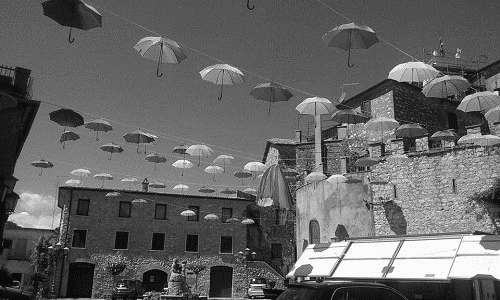
\includegraphics{img/gray-obraz1}	
	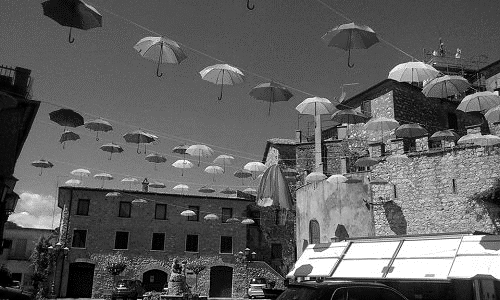
\includegraphics{img/arytmetyczne/sumowanie_stala-gray}
	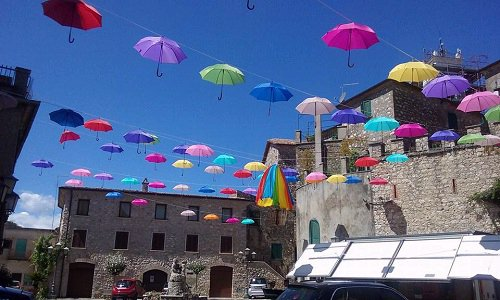
\includegraphics{img/rgb-obraz1}	
	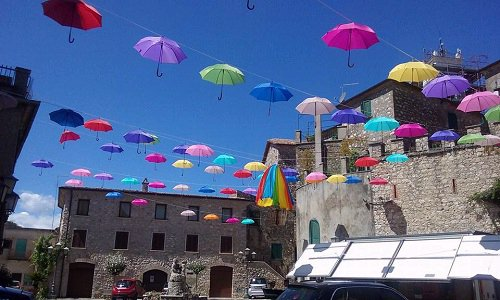
\includegraphics{img/arytmetyczne/sumowanie_stala-rgb}
	\caption{Przykład wykonania operacji dodawania stałej do obrazu - po lewej obraz przed operacją, po prawej obraz po operacji. Wartość stałej: 50 }
	\label{fig1}	
	\end{figure}
	
	
	\subsection{Sumowanie dwóch obrazów}
	Do wartości każdego piksla obrazu pierwszego dodaje wartość piksla o odpowiadających mu współrzędnych obrazu drugiego. Obsługuje obrazy szare i kolorowe.
	
	\begin{verbatim}
	public static PCXImage addImages(PCXImage inputImage1, PCXImage inputImage2) throws Exception {
        PixelsMatrix inputMatrix1 = new PixelsMatrix(inputImage1);
        PixelsMatrix inputMatrix2 = new PixelsMatrix(inputImage2);
        PixelsMatrix outputMatrix = new PixelsMatrix(inputImage1);
        outputMatrix.clear();
        for (int row = 0; row < inputImage1.getHeight(); row++) {
            for (int col = 0; col < inputImage1.getWidth(); col++) {
                switch (inputImage1.getType()) {
                    case GRAY8: {
                        int newValue = inputMatrix1.getPixelAt(col, row) + inputMatrix2.getPixelAt(col, row);
                        outputMatrix.setPixelAt(col, row, newValue);
                    }
                    break;
                    case RGB24: {
                        int newR = inputMatrix1.getPixelRat(col, row) + inputMatrix2.getPixelRat(col, row);
                        int newG = inputMatrix1.getPixelGat(col, row) + inputMatrix2.getPixelGat(col, row);
                        int newB = inputMatrix1.getPixelBat(col, row) + inputMatrix2.getPixelBat(col, row);
                        outputMatrix.setPixelAt(col, row, newR, newG, newB);
                    }
                    break;
                    default: throw new Exception("Operacja niezdefiniowana dla tego typu obrazu!");
                }
            }
        }
        return new PCXImage(outputMatrix.getImageBytes(), inputImage1);
    }
	\end{verbatim}
	
	\begin{figure}[!ht]	
	\centering	
	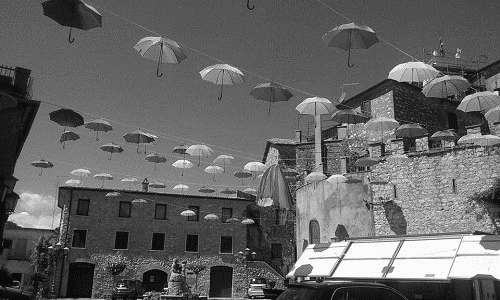
\includegraphics[width=.3\textwidth]{img/gray-obraz1}\hfill	
	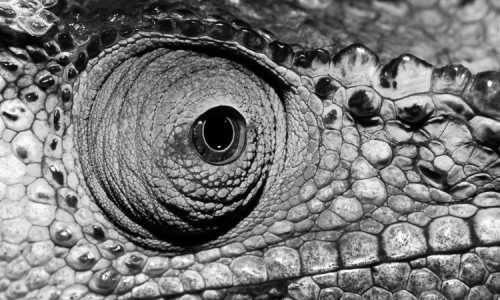
\includegraphics[width=.3\textwidth]{img/gray-obraz2}\hfill	
	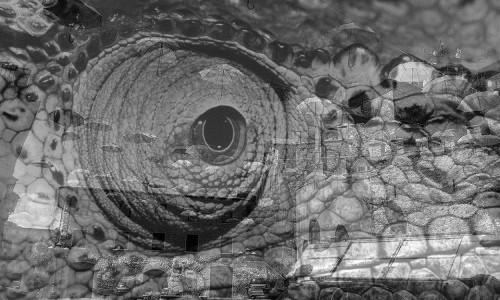
\includegraphics[width=.3\textwidth]{img/arytmetyczne/sumowanie_obrazow-gray}
	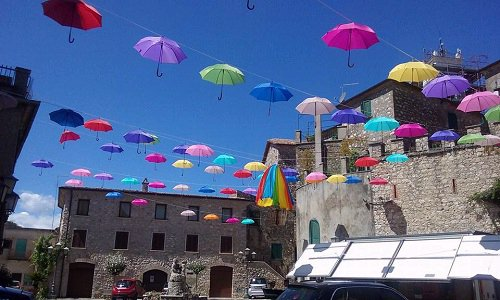
\includegraphics[width=.3\textwidth]{img/rgb-obraz1}\hfill	
	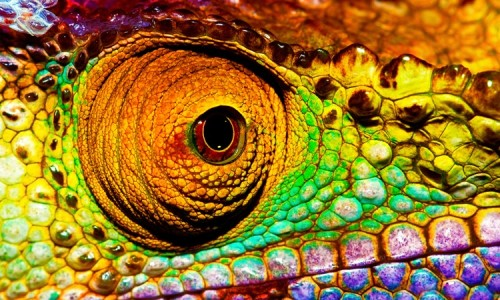
\includegraphics[width=.3\textwidth]{img/rgb-obraz2}\hfill
	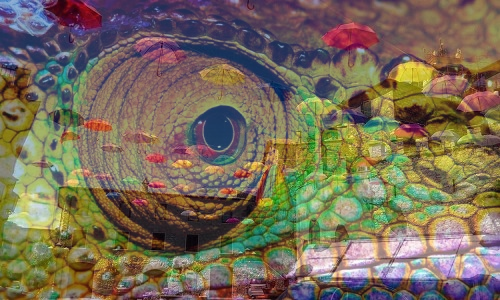
\includegraphics[width=.3\textwidth]{img/arytmetyczne/sumowanie_obrazow-rgb}
	\caption{Przykład wykonania operacji sumowania obrazów. Kolejność od lewej: obrazy wejściowe pierwszy i drugi, obraz wynikowy }
	\label{fig2}	
	\end{figure}
 

	\subsection{Mnożenie obrazu przez zadaną liczbę}
	Mnoży wartość każdego piksla obrazu przez zadaną liczbę. Obsługuje obrazy szare i kolorowe.
	
	\begin{verbatim}
	public static PCXImage multiplyImageByValue(PCXImage inputImage1, double value) throws Exception {
        PixelsMatrix inputMatrix = new PixelsMatrix(inputImage1);
        PixelsMatrix outputMatrix = new PixelsMatrix(inputImage1);
        outputMatrix.clear();
        for (int row = 0; row < inputImage1.getHeight(); row++) {
            for (int col = 0; col < inputImage1.getWidth(); col++) {
                switch (inputImage1.getType()) {
                    case GRAY8: {
                        int newValue = (int) (inputMatrix.getPixelAt(col, row) * value);
                        outputMatrix.setPixelAt(col, row, newValue);
                    }
                    break;
                    case RGB24: {
                        int newR = (int) (inputMatrix.getPixelRat(col, row) * value);
                        int newG = (int) (inputMatrix.getPixelGat(col, row) * value);
                        int newB = (int) (inputMatrix.getPixelBat(col, row) * value);

                        outputMatrix.setPixelAt(col, row, newR, newG, newB);
                    }
                    break;
                    default: throw new Exception("Operacja niezdefiniowana dla tego typu obrazu!");
                }
            }
        }

        return new PCXImage(outputMatrix.getImageBytes(), inputImage1);
    }
	\end{verbatim}
	
	\begin{figure}[!ht]	
	\centering	
	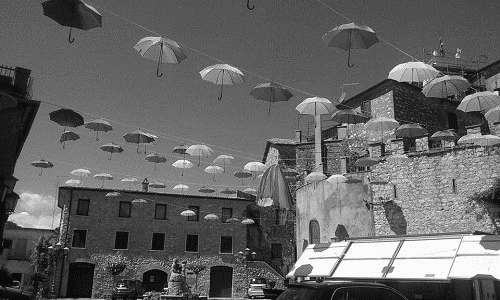
\includegraphics{img/gray-obraz1}	
	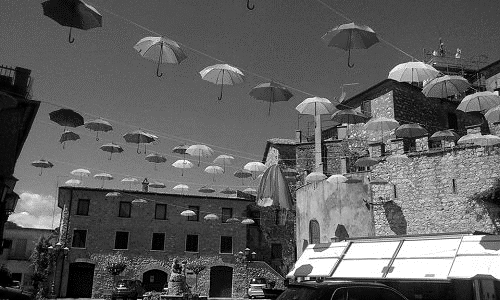
\includegraphics{img/arytmetyczne/mnozenie_stala-gray}
	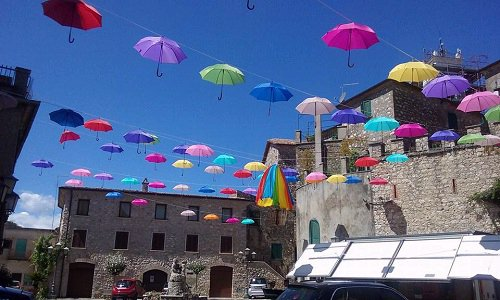
\includegraphics{img/rgb-obraz1}	
	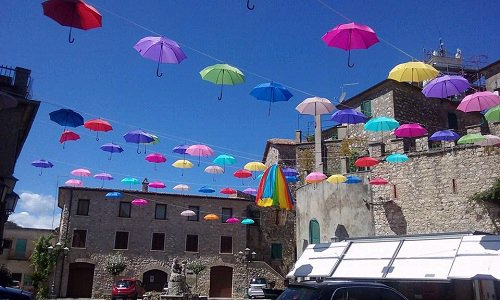
\includegraphics{img/arytmetyczne/mnozenie_stala-rgb}
	\caption{Przykład wykonania operacji mnożenia przez liczbę - po lewej obraz przed operacją, po prawej obraz po operacji. Mnożnik: 1.5 }
	\label{fig3}	
	\end{figure}
	
	\subsection{Mnożenie dwóch obrazów}
	Mnoży wartość każdego piksla obrazu pierwszego przez wartość piksla o odpowiadających mu współrzędnych obrazu drugiego. Obsługuje obrazy szare i kolorowe.
	
	\begin{verbatim}
	public static PCXImage multiplyImages(PCXImage inputImage1, PCXImage inputImage2) throws Exception {
        PixelsMatrix inputMatrix1 = new PixelsMatrix(inputImage1);
        PixelsMatrix inputMatrix2 = new PixelsMatrix(inputImage2);
        PixelsMatrix outputMatrix = new PixelsMatrix(inputImage1);
        outputMatrix.clear();

        for (int row = 0; row < inputImage1.getHeight(); row++) {
            for (int col = 0; col < inputImage1.getWidth(); col++) {
                switch (inputImage1.getType()) {
                    case GRAY8: {
                        int newValue = inputMatrix1.getPixelAt(col, row) * inputMatrix2.getPixelAt(col, row);
                        outputMatrix.setPixelAt(col, row, newValue);
                    }
                    break;
                    case RGB24: {
                        int newR = inputMatrix1.getPixelRat(col, row) * inputMatrix2.getPixelRat(col, row);
                        int newG = inputMatrix1.getPixelGat(col, row) * inputMatrix2.getPixelGat(col, row);
                        int newB = inputMatrix1.getPixelBat(col, row) * inputMatrix2.getPixelBat(col, row);
                        outputMatrix.setPixelAt(col, row, newR, newG, newB);
                    }
                    break;
                    default: throw new Exception("Operacja niezdefiniowana dla tego typu obrazu!");
                }
            }
        }

        return new PCXImage(outputMatrix.getImageBytes(), inputImage1);
    }
	\end{verbatim}


	\begin{figure}[!ht]	
	\centering	
	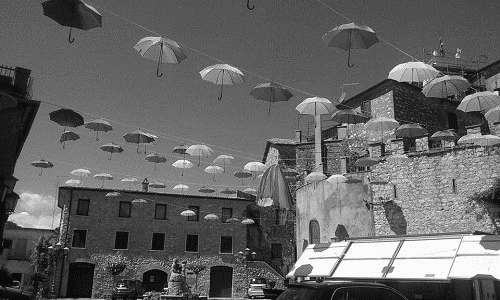
\includegraphics[width=.3\textwidth]{img/gray-obraz1}\hfill	
	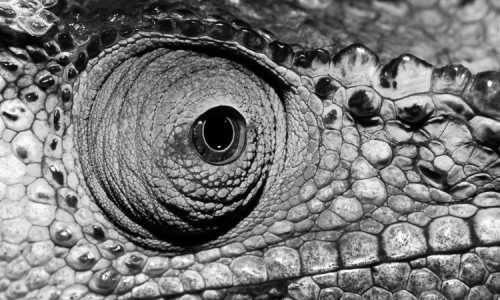
\includegraphics[width=.3\textwidth]{img/gray-obraz2}\hfill	
	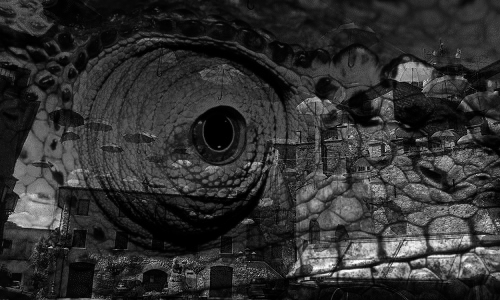
\includegraphics[width=.3\textwidth]{img/arytmetyczne/mnozenie_obrazow-gray}
	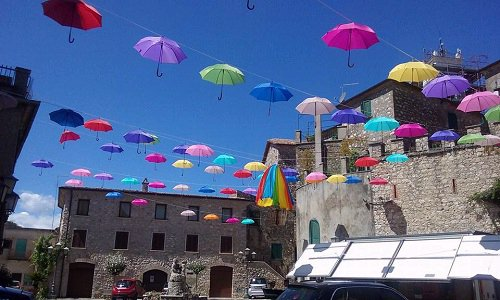
\includegraphics[width=.3\textwidth]{img/rgb-obraz1}\hfill	
	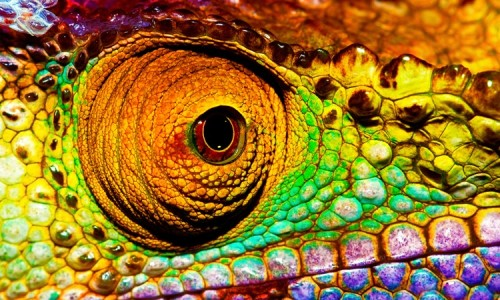
\includegraphics[width=.3\textwidth]{img/rgb-obraz2}\hfill
	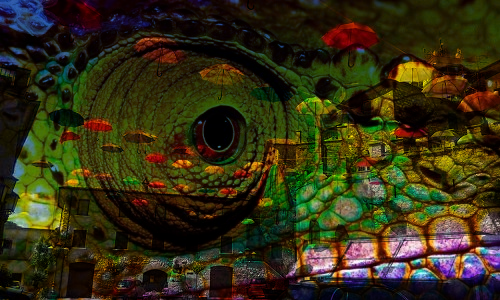
\includegraphics[width=.3\textwidth]{img/arytmetyczne/mnozenie_obrazow-rgb}
	\caption{Przykład wykonania operacji mnożenia dwóch obrazów. Kolejność od lewej: obrazy wejściowe pierwszy i drugi, obraz wynikowy }
	\label{fig4}	
	\end{figure}
	
	
	\subsection{Mieszanie obrazów z określonym współczynnikiem}
	\begin{equation*}
	f_{i}' := (\alpha * f_{i})+((1-\alpha)*f_{i}), dla \alpha\in[0, 1]
	\end{equation*}
	Obsługuje obrazy szare i kolorowe.
	
	\begin{verbatim}
	    public static PCXImage mixImages(PCXImage inputImage1, PCXImage inputImage2, double alpha) throws Exception {
        PixelsMatrix inputMatrix1 = new PixelsMatrix(inputImage1);
        PixelsMatrix inputMatrix2 = new PixelsMatrix(inputImage2);
        PixelsMatrix outputMatrix = new PixelsMatrix(inputImage1);
        outputMatrix.clear();

        for (int row = 0; row < inputImage1.getHeight(); row++) {
            for (int col = 0; col < inputImage1.getWidth(); col++) {
                switch (inputImage1.getType()) {
                    case GRAY8: {
                        int newValue = (int) (alpha * inputMatrix1.getPixelAt(col, row) + ((1 - alpha) * inputMatrix2.getPixelAt(col, row)));
                        outputMatrix.setPixelAt(col, row, newValue);
                    }
                    break;
                    case RGB24: {
                        int newR = (int) (alpha * inputMatrix1.getPixelRat(col, row) + ((1 - alpha) * inputMatrix2.getPixelRat(col, row)));
                        int newG = (int) (alpha * inputMatrix1.getPixelGat(col, row) + ((1 - alpha) * inputMatrix2.getPixelGat(col, row)));
                        int newB = (int) (alpha * inputMatrix1.getPixelBat(col, row) + ((1 - alpha) * inputMatrix2.getPixelBat(col, row)));

                        outputMatrix.setPixelAt(col, row, newR, newG, newB);
                    }
                    break;
                    default: throw new Exception("Operacja niezdefiniowana dla tego typu obrazu!");
                }
            }
        }

        return new PCXImage(outputMatrix.getImageBytes(), inputImage1);

    }
	\end{verbatim}
	
	\begin{figure}[!ht]	
	\centering	
	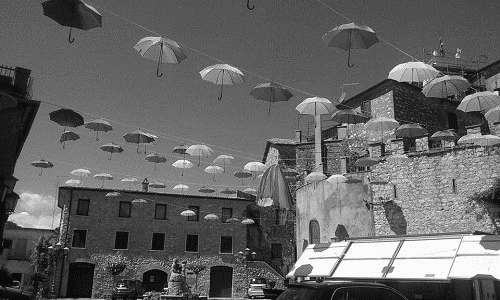
\includegraphics[width=.3\textwidth]{img/gray-obraz1}\hfill	
	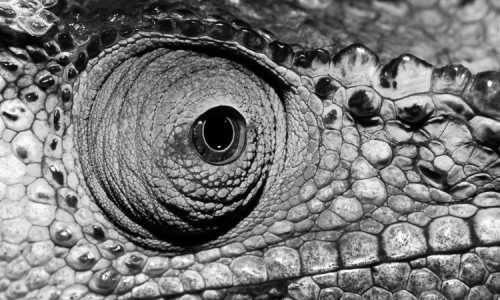
\includegraphics[width=.3\textwidth]{img/gray-obraz2}\hfill	
	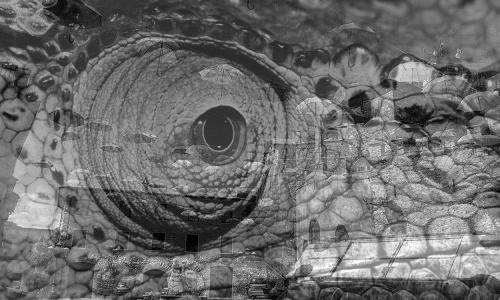
\includegraphics[width=.3\textwidth]{img/arytmetyczne/mieszanie-gray}
	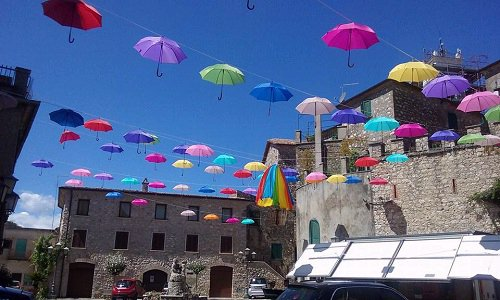
\includegraphics[width=.3\textwidth]{img/rgb-obraz1}\hfill	
	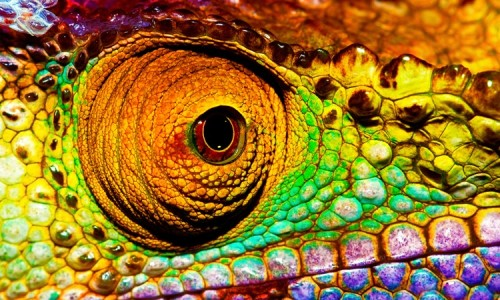
\includegraphics[width=.3\textwidth]{img/rgb-obraz2}\hfill
	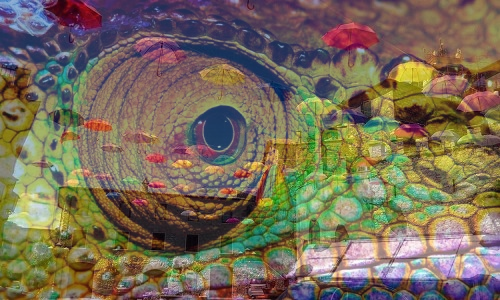
\includegraphics[width=.3\textwidth]{img/arytmetyczne/mieszanie-rgb}
	\caption{Przykład wykonania operacji mieszania dwóch obrazów ze współczynnikiem alpha=0.5. Kolejność od lewej: obrazy wejściowe pierwszy i drugi, obraz wynikowy }
	\label{fig5}	
	\end{figure}
	
	
	\subsection{Potęgowanie obrazu z zadaną potęgą}
	Dla każdego piksla w obrazie wejściowym podnosi jego wartość do potęgi podanej przez użytkownika (argument metody: exponent).
	\begin{equation*}
	f_{i}' = f_{i}^\alpha, \alpha >0
	\end{equation*}
	Obsługuje obrazy szare i kolorowe.
	
	\begin{verbatim}
	    public static PCXImage powerImageByValue(PCXImage inputImage1, double exponent) throws Exception {
        PixelsMatrix inputMatrix = new PixelsMatrix(inputImage1);
        PixelsMatrix outputMatrix = new PixelsMatrix(inputImage1);
        outputMatrix.clear();

        for (int row = 0; row < inputImage1.getHeight(); row++) {
            for (int col = 0; col < inputImage1.getWidth(); col++) {
                switch (inputImage1.getType()) {
                    case GRAY8: {
                        int newValue = (int) (Math.pow(inputMatrix.getPixelAt(col, row), 
												exponent));
                        outputMatrix.setPixelAt(col, row, newValue);
                    }
                    break;
                    case RGB24: {
                        int newR = (int) (Math.pow(inputMatrix.getPixelRat(col, row), 
												exponent));
                        int newG = (int) (Math.pow(inputMatrix.getPixelGat(col, row), 
												exponent));
                        int newB = (int) (Math.pow(inputMatrix.getPixelBat(col, row), 
												exponent));
                        
                        outputMatrix.setPixelAt(col, row, newR, newG, newB);
                    }
                    break;
                    default: throw new Exception("Operacja niezdefiniowana dla tego typu obrazu!");
                }
            }
        }

        return new PCXImage(outputMatrix.getImageBytes(), inputImage1);
    }
	\end{verbatim}
	
	\begin{figure}[!ht]	
	\centering	
	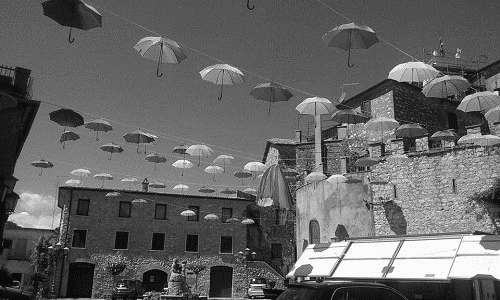
\includegraphics[scale=0.8]{img/gray-obraz1}	
	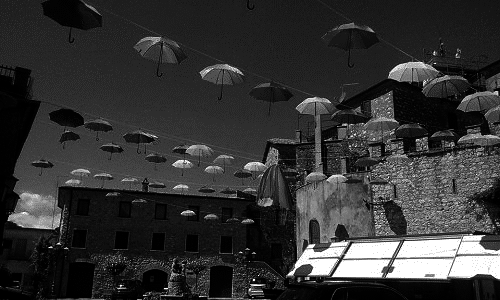
\includegraphics[scale=0.8]{img/arytmetyczne/potegowanie-gray}\\
	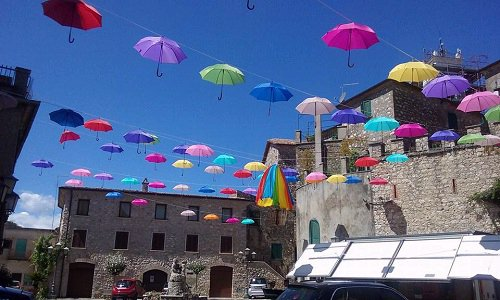
\includegraphics[scale=0.8]{img/rgb-obraz1}	
	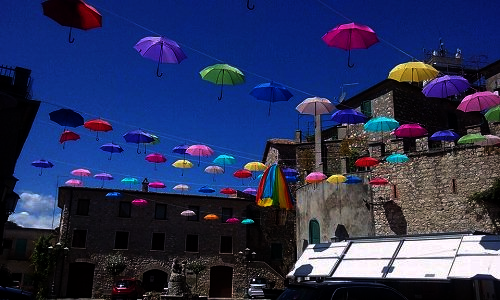
\includegraphics[scale=0.8]{img/arytmetyczne/potegowanie-rgb}
	\caption{Przykład wykonania operacji podnoszenia obrazu do potęgi 2. Po lewej obraz przed operacją, po prawej obraz po operacji.}
	\label{fig6}	
	\end{figure}
	
	
	\subsection{Pierwiastkowanie obrazu}
	Dla każdego piksla obrazu wejściowego wykonuje jego pierwiastkowanie (pierwiastek kwadratowy)
	Obsługuje obrazy szare i kolorowe.
	
	\begin{verbatim}
	static PCXImage rootImage(PCXImage plikWe1) throws Exception {
        PixelsMatrix inputMatrix = new PixelsMatrix(plikWe1);
        PixelsMatrix outputMatrix = new PixelsMatrix(plikWe1);
        outputMatrix.clear();
        
        for (int row = 0; row < inputMatrix.height; row++) {
            for (int col = 0; col < inputMatrix.width; col++) {
                switch (inputMatrix.type) {
                    case GRAY8: {
                        outputMatrix.setPixelAt(col, row, (int) (Math.sqrt(inputMatrix.getPixelAt(col, row))));
                    }
                    break;
                    case RGB24: {
                        outputMatrix.setPixelRat(col, row, (int) (Math.sqrt(inputMatrix.getPixelRat(col, row))));
                        outputMatrix.setPixelGat(col, row, (int) (Math.sqrt(inputMatrix.getPixelGat(col, row))));
                        outputMatrix.setPixelBat(col, row, (int) (Math.sqrt(inputMatrix.getPixelBat(col, row))));
                    }
                    break;
                    default: throw new Exception("Operacja niezdefiniowana dla tego typu obrazu!");
                }
            }
        }
        return new PCXImage(outputMatrix.getImageBytes(), plikWe1);
    }
	\end{verbatim}

	\begin{figure}[!ht]	
	\centering	
	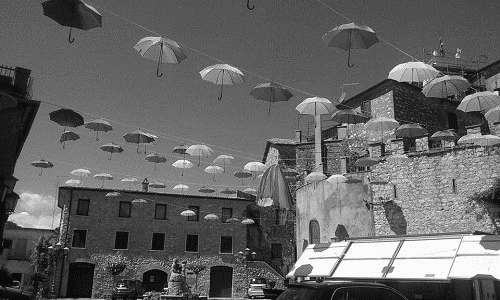
\includegraphics{img/gray-obraz1}	
	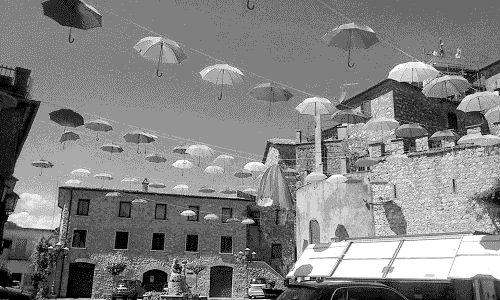
\includegraphics{img/arytmetyczne/pierwiastkowanie_obrazu-gray}
	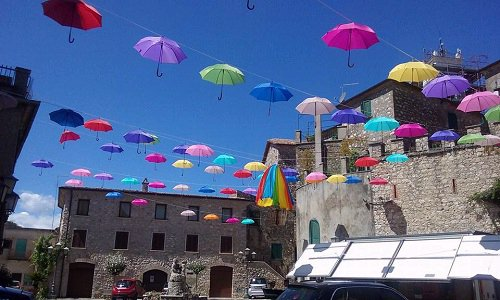
\includegraphics{img/rgb-obraz1}	
	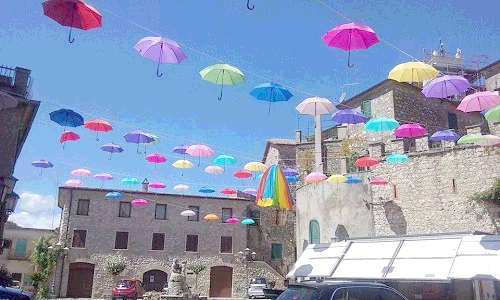
\includegraphics{img/arytmetyczne/pierwiastkowanie_obrazu-rgb}
	\caption{Przykład wykonania operacji pierwiastkowania kwadratowego.}
	\label{fig9}	
	\end{figure}
	
	
	\section{Operacje geometryczne}
	\subsection{Przemieszczenie obrazu o wektor}
	Dla każdego piksla obrazu wejściowego wykonuje jego przesunięcie o pozycję podaną w argumentach dX, dY metody.
	\begin{equation*}
	f(x,y)=f(x+dX,y+dY)
	\end{equation*}
	Obsługuje obrazy szare i kolorowe.
	
	\begin{verbatim}
	    public static PCXImage moveImageByVector(PCXImage inputImage1, int dX, int dY) throws Exception { 
        PixelsMatrix inputMatrix = new PixelsMatrix(inputImage1);

        Type type = inputMatrix.type;
        int outputWidth = inputMatrix.width;
        int outputHeight = inputMatrix.height;

        PixelsMatrix outputMatrix = new PixelsMatrix(inputImage1);
        outputMatrix.type = type;
        outputMatrix.width = outputWidth;
        outputMatrix.height = outputHeight;

        outputMatrix.clear();   //wyczysc macierz wyjsciowa

        for (int row = 0; row < inputMatrix.height; row++) {
            for (int col = 0; col < inputMatrix.width; col++) {
                int newX = col + dX;
                int newY = row + dY;

                if ((newY > 0 && newY < outputHeight) && (newX > 0 && newX < outputWidth)){//jezeli nie przekroczono zakresu przesunieciem
                    switch (type) {
                        case MONOB:
                        case GRAY8:
                            outputMatrix.setPixelAt(newX, newY, inputMatrix.getPixelAt(col, 
														row));
                            break;
                        case RGB24:
                            outputMatrix.setPixelAt(newX, newY, inputMatrix.getPixelRat(col, 
														row), inputMatrix.getPixelGat(col, row), inputMatrix.getPixelBat(col, row));
                            break;
                    }
                }
            }
        }
        return new PCXImage(outputMatrix.getImageBytes(), inputImage1);
    }
	\end{verbatim}

	\begin{figure}[!ht]	
	\centering	
	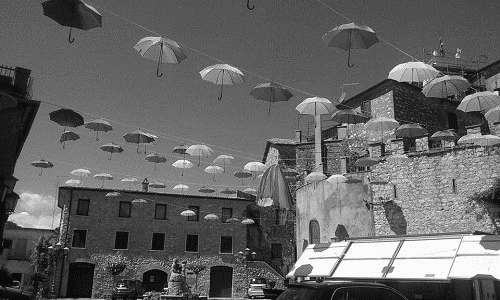
\includegraphics{img/gray-obraz1}	
	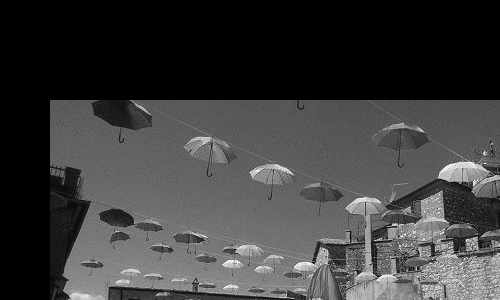
\includegraphics{img/geometryczne/przemieszczanie-gray}
	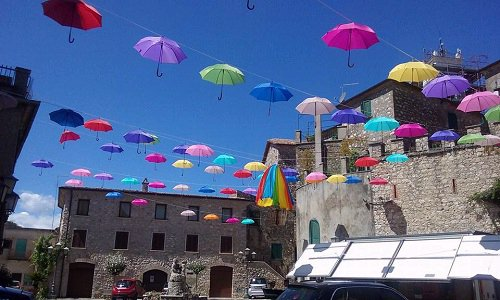
\includegraphics{img/rgb-obraz1}	
	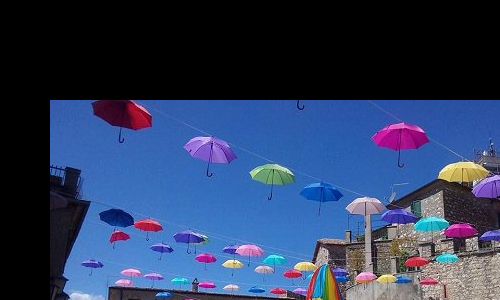
\includegraphics{img/geometryczne/przemieszczanie-rgb}
	\caption{Przykład wykonania operacji przesunięcia obrazu o wektor x=50, y=100}
	\label{fig10}	
	\end{figure}
	
	
	\subsection{Skalowanie obrazu - jednorodne i niejednorodne}
	Algorytm mnoży współrzędne każdego piksla przez współczynniki skalowania sX, sY:
	\begin{equation*}
	f(x,y)=f(x*sX,y*sY)
	\end{equation*}
	Obsługuje obrazy szare i kolorowe.
	\begin{verbatim}
	    public static PCXImage scaleImage(PCXImage inputImage1, double sX, double sY) throws Exception {
        ArrayList<Integer> imageBytes = new ArrayList<Integer>();
        ArrayList<Integer> outputBytes = new ArrayList<Integer>();

        int oldWidth = inputImage1.getWidth();
        int oldHeight = inputImage1.getHeight();
        int newWidth = (int) Math.ceil(oldWidth * sX);
        int newHeight = (int) Math.ceil(oldHeight * sY);
        int bytesPerLine = inputImage1.getBytesPerLine();

        for (int row = 0; row < newHeight; row++) {
            for (int col = 0; col < newWidth; col++) {
                double baseX = col * (double) oldWidth / newWidth;
                double baseY = row * (double) oldHeight / newHeight;

                int newCol = (int) Math.floor(baseX);
                int newRow = (int) Math.floor(baseY);
                double dx = baseX - newCol;
                double dy = baseY - newRow;
                int x, y;
                if (newCol > oldWidth) {
                    x = newCol;
                } else {
                    x = newCol + 1;
                }
                if (newRow > oldHeight) {
                    y = newRow;
                } else {
                    y = newRow + 1;
                }
                double result = (1 - dy) * imageBytes.get(newRow * bytesPerLine + newCol) 
								* (1 - dx) + imageBytes.get(y * bytesPerLine + newCol)
                        * dx + imageBytes.get(y * bytesPerLine + newCol) * (1 - dx) + 
												imageBytes.get(y * bytesPerLine + x) * dx * dy;

                outputBytes.add((int) result);
            }
        }

        PCXImage tmp = new PCXImage(inputImage1);
        tmp.setResolution(newWidth, newHeight);
        return new PCXImage(outputBytes, tmp);
    }
	\end{verbatim}
	
	\begin{figure}[!ht]	
	\centering	
	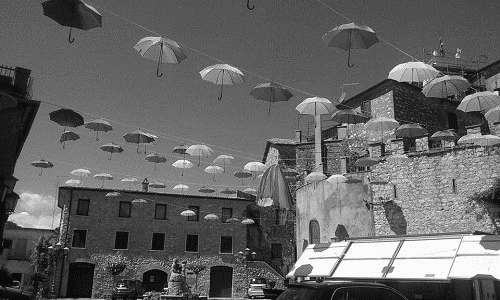
\includegraphics[scale=0.7]{img/gray-obraz1}	
	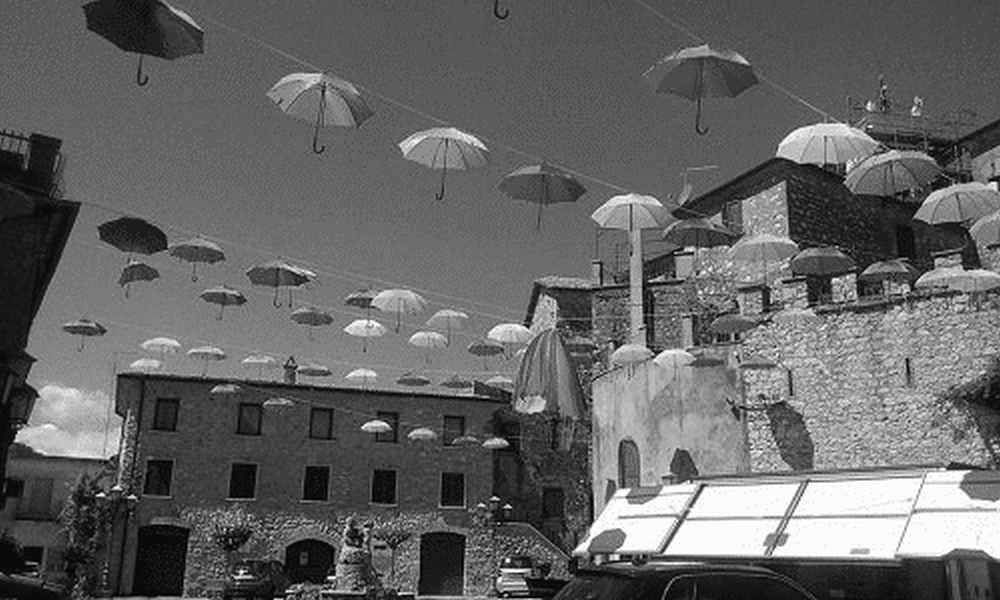
\includegraphics[scale=0.7]{img/geometryczne/skalowanie_jednorodne-gray}
	
	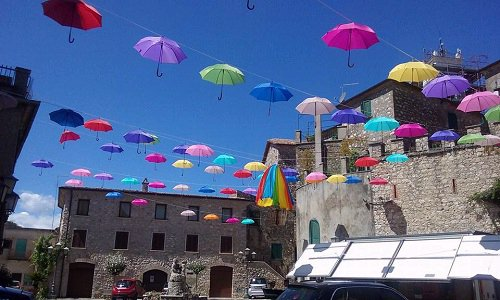
\includegraphics[scale=0.7]{img/rgb-obraz1}	
	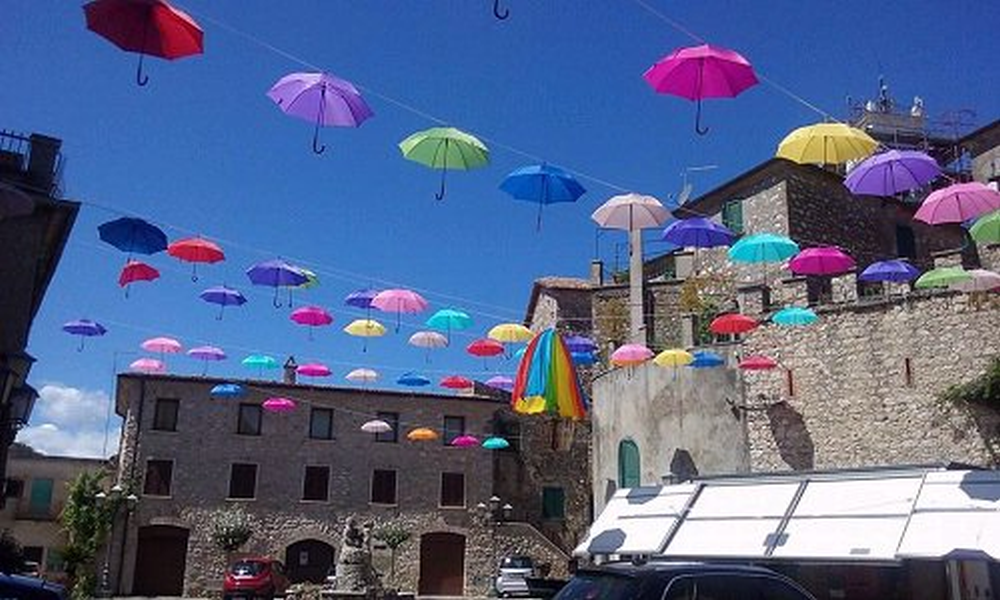
\includegraphics[scale=0.7]{img/geometryczne/skalowanie_jednorodne-rgb}
	\caption{Przykład wykonania operacji skalowania jednorodnego z parametrami x=2, y=2}
	\label{fig11}	
	\end{figure}
	
	\begin{figure}[!ht]	
	\centering	
	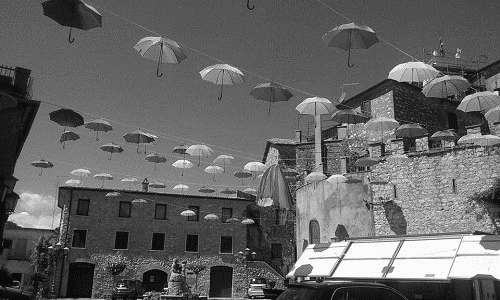
\includegraphics[scale=0.7]{img/gray-obraz1}	
	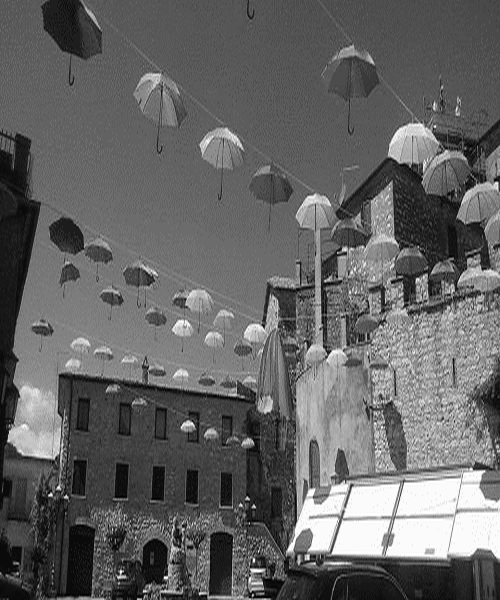
\includegraphics[scale=0.7]{img/geometryczne/skalowanie_niejednorodne-gray}
	
	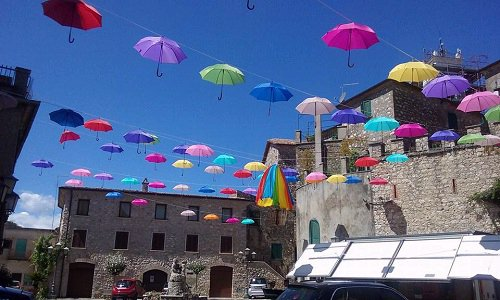
\includegraphics[scale=0.7]{img/rgb-obraz1}	
	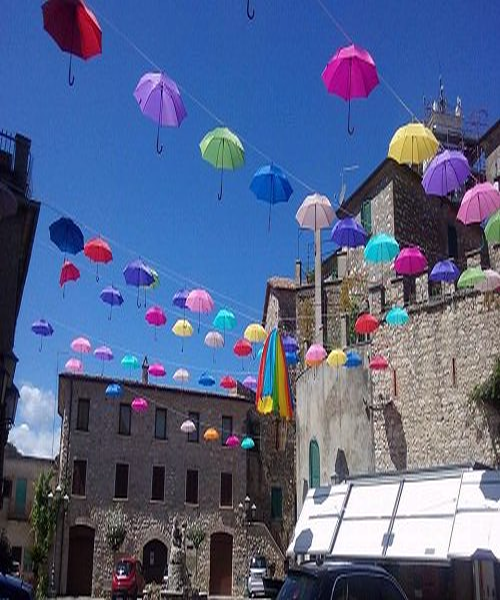
\includegraphics[scale=0.7]{img/geometryczne/skalowanie_niejednorodne-rgb}
	\caption{Przykład wykonania operacji skalowania niejednorodnego z parametrami x=1, y=2}
	\label{fig11}	
	\end{figure}

	
	\subsection{Symetria względem osi X}
	Dla każdego piksla obrazu wejściowego wykonuje jego symetryczne odbicie.
	Obsługuje obrazy szare i kolorowe.
	
	\begin{verbatim}
	    static PCXImage verticalSymmetry(PCXImage plikWe1) throws Exception {
        PixelsMatrix inputMatrix = new PixelsMatrix(plikWe1);
        PixelsMatrix outputMatrix = new PixelsMatrix(plikWe1);
        outputMatrix.clear();
        int width = plikWe1.getWidth();
        int height = plikWe1.getHeight();
        Type type = plikWe1.getType();

        for (int row = 0; row < height; row++) {
            for (int col = 0; col < width / 2; col++) {
                switch (type) {
                    case GRAY8: {
                        outputMatrix.setPixelAt(col, row, inputMatrix.getPixelAt(width - 
												col - 1, row));
                        outputMatrix.setPixelAt(width - col - 1, row, inputMatrix.getPixelAt
												(col, row));
                    }
                    break;
                    case RGB24: {
                        outputMatrix.setPixelRat(col, row, inputMatrix.getPixelRat(width -
												col - 1, row));
                        outputMatrix.setPixelRat(width - col - 1, row, inputMatrix.getPixelRat
												(col, row));

                        outputMatrix.setPixelGat(col, row, inputMatrix.getPixelGat(width -
												col - 1, row));
                        outputMatrix.setPixelGat(width - col - 1, row, inputMatrix.getPixelGat
												(col, row));

                        outputMatrix.setPixelBat(col, row, inputMatrix.getPixelBat(width -
												col - 1, row));
                        outputMatrix.setPixelBat(width - col - 1, row, inputMatrix.getPixelBat
												(col, row));
                    }
                    break;
                    default:
                        throw new Exception("Symetria w poziomie obsługiwana tylko dla obrazów szarych i kolorowych!");
                }
            }
        }
        return new PCXImage(outputMatrix.getImageBytes(), plikWe1);
    }
	\end{verbatim}

	\begin{figure}[!ht]	
	\centering	
	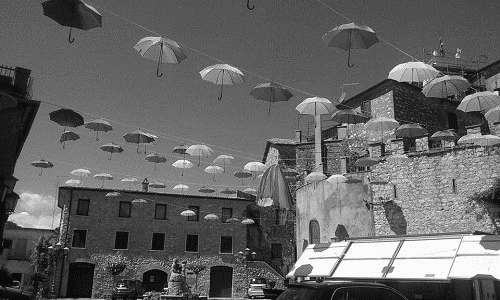
\includegraphics{img/gray-obraz1}	
	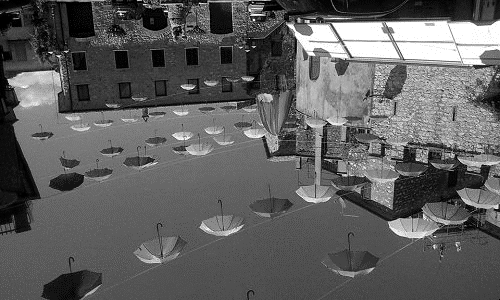
\includegraphics{img/geometryczne/symetriaX-gray}
	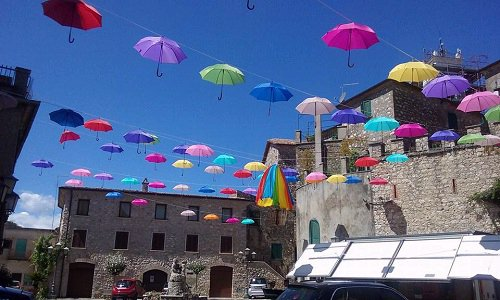
\includegraphics{img/rgb-obraz1}	
	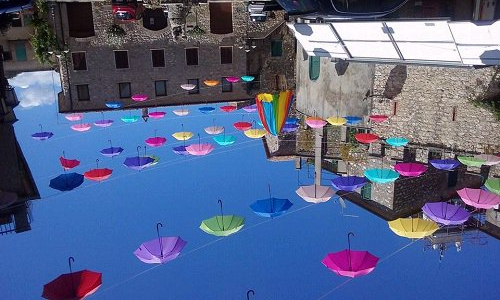
\includegraphics{img/geometryczne/symetriaX-rgb}
	\caption{Przykład wykonania operacji operacji symetrii względem osi X}
	\label{fig11}	
	\end{figure}
	
	
	\subsection{Symetria względem osi Y}
	Dla każdego piksla obrazu wejściowego wykonuje jego symetryczne odbicie.
	Obsługuje obrazy szare i kolorowe.
	
	\begin{verbatim}
	static PCXImage horizontalSymmetry(PCXImage plikWe1) throws Exception {
        PixelsMatrix inputMatrix = new PixelsMatrix(plikWe1);
        PixelsMatrix outputMatrix = new PixelsMatrix(plikWe1);
        outputMatrix.clear();
        int width = plikWe1.getWidth();
        int height = plikWe1.getHeight();
        Type type = plikWe1.getType();

        for (int row = 0; row < height / 2; row++) {
            for (int col = 0; col < width; col++) {
                switch (type) {
                    case GRAY8: {
                        outputMatrix.setPixelAt(col, row, inputMatrix.getPixelAt(col, height - row - 1));
                        outputMatrix.setPixelAt(col, height - row - 1, inputMatrix.getPixelAt(col, row));
                    }
                    break;
                    case RGB24: {
                        outputMatrix.setPixelRat(col, row, inputMatrix.getPixelRat(col, height - row - 1));
                        outputMatrix.setPixelRat(col, height - row - 1, inputMatrix.getPixelRat(col, row));

                        outputMatrix.setPixelGat(col, row, inputMatrix.getPixelGat(col, height - row - 1));
                        outputMatrix.setPixelGat(col, height - row - 1, inputMatrix.getPixelGat(col, row));

                        outputMatrix.setPixelBat(col, row, inputMatrix.getPixelBat(col, height - row - 1));
                        outputMatrix.setPixelBat(col, height - row - 1, inputMatrix.getPixelBat(col, row));
                    }
                    break;
                    default:
                        throw new Exception("Symetria w pionie obsługiwana tylko dla obrazów szarych i kolorowych!");
                }
            }
        }
        return new PCXImage(outputMatrix.getImageBytes(), plikWe1);
    }
	\end{verbatim}

	\begin{figure}[!ht]	
	\centering	
	\includegraphics{img/gray-obraz1}	
	\includegraphics{img/geometryczne/symetriaY-gray}
	\includegraphics{img/rgb-obraz1}	
	\includegraphics{img/geometryczne/symetriaY-rgb}
	\caption{Przykład wykonania operacji operacji symetrii względem osi Y}
	\label{fig12}	
	\end{figure}
	
	
	\subsection{Wycinanie fragmentów obrazu}
	Dla każdego piksla obrazu wejściowego z zakresu podanego w argumentach x1,y1 i x2,y2 zamalowuje go na czarno.
	Obsługuje obrazy szare i kolorowe.
	
	\begin{verbatim}
    static PCXImage cutImageFragment(PCXImage plikWe1, int x1, int y1, int x2, int y2) throws Exception {
        PixelsMatrix inputMatrix = new PixelsMatrix(plikWe1);
        PixelsMatrix outputMatrix = new PixelsMatrix(plikWe1);  //przepisz wszystko
        //outputMatrix.clear();
        Type type = inputMatrix.type;
        int width = plikWe1.getWidth();
        int height = plikWe1.getWidth();

        for (int row = y1; row < y2; row++) {
            for (int col = x1; col < x2; col++) {
                switch (type) {
                    case GRAY8: {
                        outputMatrix.setPixelAt(col, row, 0);
                    }
                    break;
                    case RGB24: {
                        outputMatrix.setPixelRat(col, row, 0);
                        outputMatrix.setPixelGat(col, row, 0);
                        outputMatrix.setPixelBat(col, row, 0);
                    }
                    break;
                    default:
                        throw new Exception("Wycinianie obrazu obsługiwane tylko dla obrazów szarych i kolorowych!");
                }
            }
        }
        return new PCXImage(outputMatrix.getImageBytes(), plikWe1);
    }
	\end{verbatim}

	\begin{figure}[!ht]	
	\centering	
	\includegraphics{img/gray-obraz1}	
	\includegraphics{img/geometryczne/wycinanie-gray}
	\includegraphics{img/rgb-obraz1}	
	\includegraphics{img/geometryczne/wycinanie-rgb}
	\caption{Przykład wykonania operacji operacji wycinania fragmentów obrazu x1=y1=50, x2=y2=150}
	\label{fig13}	
	\end{figure}
	
	
	\subsection{Kopiowanie fragmentów obrazu}
	Dla każdego piksla obrazu wejściowego z zakresu podanego w argumentach x1,y1 i x2,y2 przepisuje go w obrazie wyjściowym.
	Obsługuje obrazy szare i kolorowe.
	
	\begin{verbatim}
        static PCXImage copyImageFragment(PCXImage plikWe1, int x1, int y1, int x2, int y2) throws Exception {
        PixelsMatrix inputMatrix = new PixelsMatrix(plikWe1);
        PixelsMatrix outputMatrix = new PixelsMatrix(plikWe1);
        outputMatrix.clear();
        Type type = inputMatrix.type;

        for (int row = y1; row < y2; row++) {
            for (int col = x1; col < x2; col++) {
                switch (type) {
                    case GRAY8: {
                        outputMatrix.setPixelAt(col, row, inputMatrix.getPixelAt(col, row));
                    }
                    break;
                    case RGB24: {
                        outputMatrix.setPixelRat(col, row, inputMatrix.getPixelRat(col, row));
                        outputMatrix.setPixelGat(col, row, inputMatrix.getPixelGat(col, row));
                        outputMatrix.setPixelBat(col, row, inputMatrix.getPixelBat(col, row));
                    }
                    break;
                    default:
                        throw new Exception("Wycinianie obrazu obsługiwane tylko dla obrazów szarych i kolorowych!");
                }
            }
        }
        return new PCXImage(outputMatrix.getImageBytes(), plikWe1);
    }
	\end{verbatim}

	\begin{figure}[!ht]	
	\centering	
	\includegraphics{img/gray-obraz1}	
	\includegraphics{img/geometryczne/kopiowanie-gray}
	\includegraphics{img/rgb-obraz1}	
	\includegraphics{img/geometryczne/kopiowanie-rgb}
	\caption{Przykład wykonania operacji operacji kopiowania fragmentów obrazu x1=y1=50, x2=y2=150}
	\label{fig14}	
	\end{figure}
	
	
	
	
	
  \section{Operacje na histogramie}
	\subsection{Obliczanie histogramu}
	Algorytm dla każdego piksla zwiększa o 1 indeks tablicy, który odpowiada wartości piksla. Dane są następnie zapisywane w pliku tekstowym, który załadowałem do programu rysującego wykresy na podstawie danych: Gnuplot.
	\begin{verbatim}
	public static void countHistogram(PCXImage inputFile1) throws Exception {
        initTabs();
        Type type = inputFile1.getType();
        ArrayList<Integer> imageBytes = inputFile1.getDecodedImageBytes();
        int width = inputFile1.getWidth();
        int height = inputFile1.getHeight();

        log("liczenie histogramu dla obrazu " + type.toString());
        switch (inputFile1.getType()) {
            case GRAY8: {
                for (int i = 0; i < imageBytes.size(); i++) {
                    (grayHistogram[imageBytes.get(i)])++;
                }
            }
            break;
            case RGB24: {
                PixelsMatrix pixelsMatrix = new PixelsMatrix(inputFile1);

                for (int row = 0; row < height; row++) {
                    for (int col = 0; col < width; col++) {
                        rgbHistogram[0][pixelsMatrix.getPixelRat(col, row)]++;  //red
                        rgbHistogram[1][pixelsMatrix.getPixelGat(col, row)]++;  //green
                        rgbHistogram[2][pixelsMatrix.getPixelBat(col, row)]++;  //blue
                    }
                }
            }
            break;
            default:
                Tool.error("Histogram moze byc liczony tylko dla obrazow rgb24 i gray8!");
                break;
        }
        isHistogramValid(inputFile1);

        showHistogram(type);
    }
	\end{verbatim}
	
	\begin{figure}[!ht]	
	\centering	
	\includegraphics[scale=2]{img/gray-obraz1}	
	\includegraphics[scale=0.4]{img/histogram/obliczanie-gray}
	\caption{Przykład obliczonego histogramu obrazu szarego}
	\label{fig15}	
	\end{figure}	
	
  \begin{figure}[!ht]	
	\centering	
	\includegraphics[scale=2]{img/histogram/obliczanie-rgb}
	\includegraphics[scale=0.3]{img/histogram/obliczanie-r}
  \includegraphics[scale=0.3]{img/histogram/obliczanie-g}
	\includegraphics[scale=0.3]{img/histogram/obliczanie-b}
	\caption{Przykład obliczonego histogramu obrazu kolorowego}
	\label{fig16}	
	\end{figure}	
	
	
	\subsection{Rozciąganie histogramu}
	Rozciąga zakres wartości pikseli do [0, 255]. 
	\begin{equation*}
	f':=255*\frac{f-f_{min}}{f_{max}-f_{min}}
	\end{equation*}
	\begin{verbatim}
public static PCXImage stretchHistogram(PCXImage inputImage1) throws Exception {
        PixelsMatrix inputMatrix = new PixelsMatrix(inputImage1);
        PixelsMatrix outputMatrix = new PixelsMatrix(inputImage1, false);
        
        int width = inputMatrix.width;
        int height = inputMatrix.height;
        Type type = inputMatrix.type;
        int min = PCXImage.findMin(inputMatrix.getImageBytes());
        int max = PCXImage.findMax(inputMatrix.getImageBytes());

        try {
            for (int row = 0; row < height; row++) {
                for (int col = 0; col < width; col++) {
                    switch (type) {
                        case GRAY8: {
                            int newValue = (inputMatrix.getPixelAt(col, row) - min) * 255 / (max - min);
                            outputMatrix.setPixelAt(col, row, newValue);
                        }
                        break;
                        case RGB24: {
                            int r = ((inputMatrix.getPixelRat(col, row) - min) * 255) / (max - min);
                            int g = ((inputMatrix.getPixelGat(col, row) - min) * 255) / (max - min);
                            int b = ((inputMatrix.getPixelBat(col, row) - min) * 255) / (max - min);
                            outputMatrix.setPixelAt(col, row, r, g, b);
                        }
                        break;
                        default:
                            throw new Exception("Rozciaganie histogramu obsługuje tylko gray i rgb");
                    }
                }
            }
        } catch (ArithmeticException e) {
            Tool.error("Próba dzielenia przez zero!");
        }
        return new PCXImage(outputMatrix.getImageBytes(), inputImage1);
    }

	\end{verbatim}
	
	\begin{figure}[!ht]	
	\centering	
	\includegraphics[scale=1.2]{img/histogram/nierozciagniety-gray}
	\includegraphics[scale=1.2]{img/histogram/rozciagniety-gray}
	
  \includegraphics[scale=1.2]{img/histogram/nierozciagniety-rgb}
	\includegraphics[scale=1.2]{img/histogram/rozciagniety-rgb}
	\caption{Przykład rozciągania histogramu}
	\label{fig16}	
	\end{figure}	


	\section{Operacje morfologiczne}
	\subsection{Erozja (okrawanie)}
	Dla każdego piksla w macierzy obrazu, sprawdza jego 4-sąsiadów i przypisuje mu wartość najmniejszego z nich.
	Obsługuje obrazy monochromatyczne i szare.
	
	\begin{verbatim}
  public static PCXImage erodeImage(PCXImage image1) throws Exception {
        ArrayList<Integer> imageBytes = image1.getDecodedImageBytes();
        ArrayList<Integer> outputBytes = new ArrayList<Integer>(image1.getResolution());
        for (int i = 0; i < image1.getResolution(); i++) {
            outputBytes.add(0);
        }

        int width = image1.getWidth();
        int height = image1.getHeight();
        Type type = image1.getType();
        int min = 255;  //min=max

        if (type != Type.MONOB && type != Type.GRAY8) {
            throw new Exception("erozja tylko dla obrazów mono i szarych!");
        }

        for (int row = 0; row < height; row++) {
            for (int col = 0; col < width; col++) {
                min = getMinNeighborOfPixel(col, row, imageBytes, width, height);
                outputBytes.set(col + row * width, min);
            }
        }

        return new PCXImage(outputBytes, image1);
    }
	\end{verbatim}
	
	Na potrzeby algorytmu erozji napisałem metodę zwracającą wartość najmniejszego sąsiada \textbf{getMinNeighbotOfPixel(col, row, imageBytes, width, height)}:
	\begin{verbatim}
	    public static int getMinNeighborOfPixel(int col, int row, ArrayList<Integer> imageBytes, int width, int height) throws Exception {
        ArrayList<Integer> neighbors = new ArrayList<>();

        if (isPixelExist(col, row - 1, width, height)) {//piksel powyzej
            neighbors.add(imageBytes.get(col + (row - 1) * width));
        }

        if (isPixelExist(col + 1, row, width, height)) {   //piksel z prawej strony
            neighbors.add(imageBytes.get((col + 1) + row * width));
        }

        if (isPixelExist(col, row + 1, width, height)) {//piksel z dolu
            neighbors.add(imageBytes.get(col + (row + 1) * width));
        }

        if (isPixelExist(col - 1, row, width, height)) {    //piksel z lewej
            neighbors.add(imageBytes.get((col - 1) + row * width));
        }

        int min = neighbors.get(0);
        for (int i = 0; i < neighbors.size(); i++) {
            if (neighbors.get(i) < min) {
                min = neighbors.get(i);
            }
        }

        return min;
    }
	\end{verbatim}
	
	\begin{figure}[!ht]	
	\centering	
	\includegraphics[scale=1.2]{img/mono-obraz1}
	\includegraphics[scale=0.288]{img/morfologiczne/erozja-mono}
	
	\includegraphics[scale=1.2]{img/gray-obraz1}
	\includegraphics[scale=0.288]{img/morfologiczne/erozja-gray}
	\caption{Przykład wykonania erozji}
	\label{fig17}	
	\end{figure}	
	
	
	\subsection{Dylatacja (nakładanie)}
	Dla każdego piksla w macierzy obrazu, sprawdza jego 4-sąsiadów i przypisuje mu wartość największego z nich.
	Obsługuje obrazy monochromatyczne i szare.
	
	\begin{verbatim}
	    public static PCXImage dylateImage(PCXImage image1) throws Exception {
        ArrayList<Integer> imageBytes = image1.getDecodedImageBytes();
        ArrayList<Integer> outputBytes = new ArrayList<Integer>(image1.getResolution());
        for (int i = 0; i < image1.getResolution(); i++) {
            outputBytes.add(0);
        }

        int width = image1.getWidth();
        int height = image1.getHeight();
        Type type = image1.getType();
        int max = 0;  //min=max

        if (type != Type.MONOB && type != Type.GRAY8) {
            throw new Exception("erozja tylko dla obrazów mono i szarych!");
        }

     
        for (int row = 0; row < height; row++) {
            for (int col = 0; col < width; col++) {
                max = getMaxNeighborOfPixel(col, row, imageBytes, width, height);
                outputBytes.set(col + row * width, max);
            }
        }

        return new PCXImage(outputBytes, image1);    }
  \end{verbatim}

	Na potrzeby algorytmu dylatacji napisałem metodę zwracającą wartość największego sąsiada \textbf{getMaxNeighbotOfPixel(col, row, imageBytes, width, height)}:
	\begin{verbatim}
	    ArrayList<Integer> neighbors = new ArrayList<>();

        if (isPixelExist(col, row - 1, width, height)) {//piksel powyzej
            neighbors.add(imageBytes.get(col + (row - 1) * width));
        }

        if (isPixelExist(col + 1, row, width, height)) {   //piksel z prawej strony
            neighbors.add(imageBytes.get((col + 1) + row * width));
        }

        if (isPixelExist(col, row + 1, width, height)) {//piksel z dolu
            neighbors.add(imageBytes.get(col + (row + 1) * width));
        }

        if (isPixelExist(col - 1, row, width, height)) {    //piksel z lewej
            neighbors.add(imageBytes.get((col - 1) + row * width));
        }

        if (neighbors.isEmpty()) {
            throw new Exception("MorphologicOperations\\getMinNeighborOfPixel: brak sąsiadów?");
        }

        int max = neighbors.get(0);
        for (int i = 0; i < neighbors.size(); i++) {
            if (neighbors.get(i) > max) {
                max= neighbors.get(i);
            }
        }

        return max;
    }
	\end{verbatim}
	
	\begin{figure}[!ht]	
	\centering	
	\includegraphics[scale=1.2]{img/mono-obraz1}
	\includegraphics[scale=0.288]{img/morfologiczne/dylatacja-mono}
	
	\includegraphics[scale=1.2]{img/gray-obraz1}
	\includegraphics[scale=0.288]{img/morfologiczne/dylatacja-gray}
	\caption{Przykład wykonania dylatacji}
	\label{fig18}	
	\end{figure}	
	

	\subsection{Otwarcie}
	Jest to wykonanie na obrazie operacji erozji, a następnie dylatacji.
	Obsługuje obrazy monochromatyczne i szare.
	
	\begin{verbatim}
	    private void menuImageOpeningActionPerformed(java.awt.event.ActionEvent evt) {                                                 
        //erozja + dylatacja
        PCXImage plikTmp = null;
        try {
            plikTmp = MorphologicOperations.erodeImage(plikWe1);
        } catch (Exception ex) {
            Logger.getLogger(WPO_GUI.class.getName()).log(Level.SEVERE, null, ex);
        }
        try {
            plikWy = MorphologicOperations.dylateImage(plikTmp);
        } catch (Exception ex) {
            Logger.getLogger(WPO_GUI.class.getName()).log(Level.SEVERE, null, ex);
        }
        saveImage(plikWy);
    }  
	\end{verbatim}
	
	\begin{figure}[!ht]	
	\centering	
	\includegraphics[scale=1.2]{img/mono-obraz1}
	\includegraphics[scale=0.288]{img/morfologiczne/otwarcie-mono}
	
	\includegraphics[scale=1.2]{img/gray-obraz1}
	\includegraphics[scale=0.288]{img/morfologiczne/otwarcie-gray}
	\caption{Przykład wykonania otwarcia}
	\label{fig19}	
	\end{figure}	
	
	
	\subsection{Zamknięcie}
	Jest to wykonanie operacji dylatacji, a następnie erozji. 
	Obsługuje obrazy monochromatyczne i szare.
	
	\begin{verbatim}
	    private void menuImageClosingActionPerformed(java.awt.event.ActionEvent evt) {                                                 
        // dylatacja+erozja
        PCXImage plikTmp = null;

        try {
            plikTmp = MorphologicOperations.dylateImage(plikWe1);
        } catch (Exception ex) {
            Logger.getLogger(WPO_GUI.class.getName()).log(Level.SEVERE, null, ex);
        }
        try {
            plikWy = MorphologicOperations.erodeImage(plikTmp);
        } catch (Exception ex) {
            Logger.getLogger(WPO_GUI.class.getName()).log(Level.SEVERE, null, ex);
        }

        saveImage(plikWy);
    }              
	\end{verbatim}
	
	
  \begin{figure}[!ht]	
	\centering	
	\includegraphics[scale=1.2]{img/mono-obraz1}
	\includegraphics[scale=0.288]{img/morfologiczne/zamkniecie-mono}
	\includegraphics[scale=1.2]{img/gray-obraz1}
	\includegraphics[scale=0.288]{img/morfologiczne/zamkniecie-gray}
	\caption{Przykład wykonania zamknięcia}
	\label{fig20}	
	\end{figure}	


	\section{Filtrowania}
	Metoda wykonująca filtrowania bazujące na macierzy maskującej 3x3. Jako argumenty przyjmuje obraz wejściowy oraz wspomnianą macierz.
	\begin{verbatim}
	public static PCXImage filter(PCXImage inputImage, int[] maskMatrix) throws Exception {
        int width = inputImage.getWidth();
        int height = inputImage.getHeight();
        Type type = inputImage.getType();

        PixelsMatrix inputMatrix = new PixelsMatrix(inputImage);
        PixelsMatrix outputMatrix = new PixelsMatrix(inputImage);

        int sumaWagMaski = 0;
        for (int i = 0; i < maskMatrix.length; i++) {
            if (maskMatrix[i] == 0) {
                continue;
            }
            sumaWagMaski += maskMatrix[i];
        }
        if (sumaWagMaski == 0) {
            sumaWagMaski = 1;
        }

        switch (type) {
            case GRAY8: {
                for (int row = 0; row < height; row++) {  
                    for (int col = 0; col < width; col++) {
                        int sumaWazona = maskMatrix[0] * getPixel(Channel.GRAY, col - 1, 
												row - 1, inputMatrix)
                                + maskMatrix[1] * getPixel(Channel.GRAY, col, row - 1, 
																inputMatrix)
                                + maskMatrix[2] * getPixel(Channel.GRAY, col + 1, row -
																1, inputMatrix)
                                + maskMatrix[3] * getPixel(Channel.GRAY, col - 1, row,
																inputMatrix)
                                + maskMatrix[4] * getPixel(Channel.GRAY, col, row, 
																inputMatrix)
                                + maskMatrix[5] * getPixel(Channel.GRAY, col + 1, row, 
																inputMatrix)
                                + maskMatrix[6] * getPixel(Channel.GRAY, col - 1, row +
																1, inputMatrix)
                                + maskMatrix[7] * getPixel(Channel.GRAY, col, row + 1, 
																inputMatrix)
                                + maskMatrix[8] * getPixel(Channel.GRAY, col + 1, row +
																 1, inputMatrix);

                        outputMatrix.setPixelAt(col, row, sumaWazona / 1);
                    }
                }
            }
            break;
            case RGB24: {
                for (int row = 0; row < height; row++) {  
                    for (int col = 0; col < width; col++) {
                        //czerwony
                        int sumaWazonaR = maskMatrix[0] * getPixel(Channel.RED, col - 1,
												row - 1, inputMatrix)
                                + maskMatrix[1] * getPixel(Channel.RED, col, row - 1,
																inputMatrix)
                                + maskMatrix[2] * getPixel(Channel.RED, col + 1, row - 1,
																inputMatrix)
                                + maskMatrix[3] * getPixel(Channel.RED, col - 1, row, 
																inputMatrix)
                                + maskMatrix[4] * getPixel(Channel.RED, col, row, 
																inputMatrix)
                                + maskMatrix[5] * getPixel(Channel.RED, col + 1, row, 
																inputMatrix)
                                + maskMatrix[6] * getPixel(Channel.RED, col - 1, row + 1, 
																inputMatrix)
                                + maskMatrix[7] * getPixel(Channel.RED, col, row + 1, 
																inputMatrix)
                                + maskMatrix[8] * getPixel(Channel.RED, col + 1, row + 1, 
																inputMatrix);

                        outputMatrix.setPixelRat(col, row, sumaWazonaR / sumaWagMaski);

                        //zielony
                        int sumaWazonaG = maskMatrix[0] * getPixel(Channel.GREEN, col - 1, row - 1, 
												inputMatrix)
                                + maskMatrix[1] * getPixel(Channel.GREEN, col, row - 1, 
																inputMatrix)
                                + maskMatrix[2] * getPixel(Channel.GREEN, col + 1, row - 1, 
																inputMatrix)
                                + maskMatrix[3] * getPixel(Channel.GREEN, col - 1, row, 
																inputMatrix)
                                + maskMatrix[4] * getPixel(Channel.GREEN, col, row, 
																inputMatrix)
                                + maskMatrix[5] * getPixel(Channel.GREEN, col + 1, row, 
																inputMatrix)
                                + maskMatrix[6] * getPixel(Channel.GREEN, col - 1, row + 1, 
																inputMatrix)
                                + maskMatrix[7] * getPixel(Channel.GREEN, col, row + 1, 
																inputMatrix)
                                + maskMatrix[8] * getPixel(Channel.GREEN, col + 1, row + 1, 
																inputMatrix);

                        outputMatrix.setPixelGat(col, row, sumaWazonaG / sumaWagMaski);

                        //niebieski
                        int sumaWazonaB = maskMatrix[0] * getPixel(Channel.BLUE, col - 1, row - 1, 
												inputMatrix)
                                + maskMatrix[1] * getPixel(Channel.BLUE, col, row - 1, 
																inputMatrix)
                                + maskMatrix[2] * getPixel(Channel.BLUE, col + 1, row - 1, 
																inputMatrix)
                                + maskMatrix[3] * getPixel(Channel.BLUE, col - 1, row, 
																inputMatrix)
                                + maskMatrix[4] * getPixel(Channel.BLUE, col, row, 
																inputMatrix)
                                + maskMatrix[5] * getPixel(Channel.BLUE, col + 1, row, 
																inputMatrix)
                                + maskMatrix[6] * getPixel(Channel.BLUE, col - 1, row + 1, 
																inputMatrix)
                                + maskMatrix[7] * getPixel(Channel.BLUE, col, row + 1, 
																inputMatrix)
                                + maskMatrix[8] * getPixel(Channel.BLUE, col + 1, row + 1, 
																inputMatrix);

                        outputMatrix.setPixelBat(col, row, sumaWazonaB / sumaWagMaski);
                    }
                }
            }
            break;
            default: {
                Tool.error("Filtr zdefiniowany tylko dla obrazów szarych i RGB");
                return null;
            }

        }
        return new PCXImage(outputMatrix.getImageBytes(), inputImage);
    }
	\end{verbatim}
	
	\subsection{Filtrowanie dolnoprzepustowe}
	Wywołuje wyżej podaną metodę \textbf{filter} z argumentem, będącym macierzą 3x3:
	\begin{equation*}
	\begin{matrix}
	1 & 1 & 1 \\
	1 & 1 & 1 \\
	1 & 1 & 1
	\end{matrix}
	\end{equation*}
		
	\begin{figure}[!ht]	
	\centering	
	\includegraphics[scale=1.2]{img/gray-obraz1}
	\includegraphics[scale=1.2]{img/filtrowanie/gray-dolnoprzepustowe}
	
	\includegraphics[scale=1.2]{img/rgb-obraz1}
	\includegraphics[scale=1.2]{img/filtrowanie/rgb-dolnoprzepustowe}
	\caption{Przykład wykonania filtrowania dolnoprzepustowego}
	\label{fig21}	
	\end{figure}	
	
	
	\subsection{Filtrowanie górnoprzepustowe - Robertsa}
	Wywołuje wyżej podaną metodę \textbf{filter} z argumentem, będącym macierzą 3x3:
	\begin{equation*}
	\begin{matrix}
	0 & 0 & 0 \\
	-1 & 0 & 0 \\
	0 & 1 & 0
	\end{matrix}
	\end{equation*}
		
	\begin{figure}[!ht]	
	\centering	
	\includegraphics[scale=1.2]{img/gray-obraz1}
	\includegraphics[scale=1.2]{img/filtrowanie/gray-gornoprzepustowe-robertsa}
	
	\includegraphics[scale=1.2]{img/rgb-obraz1}
	\includegraphics[scale=1.2]{img/filtrowanie/rgb-gornoprzepustowe-robertsa}
	\caption{Przykład wykonania filtrowania górnoprzepustowego}
	\label{fig22}	
	\end{figure}	
	
	
	\subsection{Filtrowanie gradientowe - kompasowe}
	Wywołuje wyżej podaną metodę \textbf{filter} z argumentem, będącym macierzą 3x3, której zawartość zależy od kierunku filtrowania. Kierunki: N(Północ), E(wschód), SW(południowy-zachód), itd.
	Przykładowe macierze dla dwóch wybranych kierunków i wyniki realizacji dla nich algorytmu:
	\subsubsection{Macierz dla kierunku północnego:}
	\begin{equation*}
	\begin{matrix}
	1 & 1 & 1 \\
	1 & -2 & 1 \\
	-1 & -1 & -1
	\end{matrix}
	\end{equation*}
		
	\begin{figure}[!ht]	
	\centering	
	\includegraphics[scale=1.2]{img/rgb-obraz1}
	\includegraphics[scale=1.2]{img/filtrowanie/gray-gradientowekompasowe-polnoc}
	\caption{Przykład wykonania filtrowania kompasowego: kierunek północny}
	\label{fig16}	
	\end{figure}	
	
	\subsubsection{Macierz dla kierunku południowego:}
	\begin{equation*}
	\begin{matrix}
	-1 & -1 & -1 \\
	1 & -2 & 1 \\
	1 & 1 & 1
	\end{matrix}
	\end{equation*}
		
	\begin{figure}[!ht]	
	\centering	
	\includegraphics[scale=1.2]{img/rgb-obraz1}
	\includegraphics[scale=1.2]{img/filtrowanie/rgb-gradientowekompasowe-poludnie}
	\caption{Przykład wykonania filtrowania kompasowego: kierunek południowy}
	\label{fig23}	
	\end{figure}	
	
	
	\subsection{Filtrowanie górnoprzepustowe - Robertsa}
	Wywołuje wyżej podaną metodę filter z argumentem, będącym macierzą 3x3:
	\begin{equation*}
	\begin{matrix}
	0 & 0 & 0 \\
	-1 & 0 & 0 \\
	0 & 1 & 0
	\end{matrix}
	\end{equation*}
		
	\begin{figure}[!ht]	
	\centering	
	\includegraphics[scale=1.2]{img/gray-obraz1}
	\includegraphics[scale=1.2]{img/filtrowanie/gray-gornoprzepustowe-robertsa}
	
	\includegraphics[scale=1.2]{img/rgb-obraz1}
	\includegraphics[scale=1.2]{img/filtrowanie/rgb-gornoprzepustowe-robertsa}
	\caption{Przykład wykonania filtrowania górnoprzepustowego}
	\label{fig24}	
	\end{figure}	
	
	
	\subsection{Filtrowanie medianowe}
	Dla każdego piksla obrazu dodaje do uporządkowanej listy wartość jego oraz jego 8-sąsiadów, następnie sortuję ową listę rosnąco i wybiera z niej medianę - która zostaje przypisana wartości aktualnie rozpatrywanego piksela.
	\begin{verbatim}
	public static PCXImage medianFilter(PCXImage inputImage) throws Exception {
        PixelsMatrix inputMatrix = new PixelsMatrix(inputImage);
        PixelsMatrix outputMatrix = new PixelsMatrix(inputImage);
        outputMatrix.clear();
        int width = inputImage.getWidth();
        int height = inputImage.getHeight();
        Type type = inputImage.getType();

        for (int row = 0; row < height; row++) {
            for (int col = 0; col < width; col++) {
                switch (type) {
                    case GRAY8: {
                        int newValue = median(new int[]{
                                getPixel(Channel.GRAY, col - 1, row - 1, inputMatrix),
                                getPixel(Channel.GRAY, col, row - 1, inputMatrix),
                                getPixel(Channel.GRAY, col + 1, row - 1, inputMatrix),
                                getPixel(Channel.GRAY, col - 1, row, inputMatrix),
                                getPixel(Channel.GRAY, col, row, inputMatrix),
                                getPixel(Channel.GRAY, col + 1, row, inputMatrix),
                                getPixel(Channel.GRAY, col - 1, row + 1, inputMatrix),
                                getPixel(Channel.GRAY, col, row + 1, inputMatrix),
                                getPixel(Channel.GRAY, col + 1, row + 1, inputMatrix)}
                        );
                        
                        outputMatrix.setPixelAt(col, row, newValue);
                    }
                    break;
                    case RGB24: {
                        int newR = median(new int[]{
                                getPixel(Channel.RED, col - 1, row - 1, inputMatrix),
                                getPixel(Channel.RED, col, row - 1, inputMatrix),
                                getPixel(Channel.RED, col + 1, row - 1, inputMatrix),
                                getPixel(Channel.RED, col - 1, row, inputMatrix),
                                getPixel(Channel.RED, col, row, inputMatrix),
                                getPixel(Channel.RED, col + 1, row, inputMatrix),
                                getPixel(Channel.RED, col - 1, row + 1, inputMatrix),
                                getPixel(Channel.RED, col, row + 1, inputMatrix),
                                getPixel(Channel.RED, col + 1, row + 1, inputMatrix)}
                        );
                        
                        int newG = median(new int[]{
                                getPixel(Channel.GREEN, col - 1, row - 1, inputMatrix),
                                getPixel(Channel.GREEN, col, row - 1, inputMatrix),
                                getPixel(Channel.GREEN, col + 1, row - 1, inputMatrix),
                                getPixel(Channel.GREEN, col - 1, row, inputMatrix),
                                getPixel(Channel.GREEN, col, row, inputMatrix),
                                getPixel(Channel.GREEN, col + 1, row, inputMatrix),
                                getPixel(Channel.GREEN, col - 1, row + 1, inputMatrix),
                                getPixel(Channel.GREEN, col, row + 1, inputMatrix),
                                getPixel(Channel.GREEN, col + 1, row + 1, inputMatrix)}
                        );
                        
                        int newB = median(new int[]{
                                getPixel(Channel.BLUE, col - 1, row - 1, inputMatrix),
                                getPixel(Channel.BLUE, col, row - 1, inputMatrix),
                                getPixel(Channel.BLUE, col + 1, row - 1, inputMatrix),
                                getPixel(Channel.BLUE, col - 1, row, inputMatrix),
                                getPixel(Channel.BLUE, col, row, inputMatrix),
                                getPixel(Channel.BLUE, col + 1, row, inputMatrix),
                                getPixel(Channel.BLUE, col - 1, row + 1, inputMatrix),
                                getPixel(Channel.BLUE, col, row + 1, inputMatrix),
                                getPixel(Channel.BLUE, col + 1, row + 1, inputMatrix)}
                        );
                        
                        outputMatrix.setPixelAt(col, row, newR, newG, newB);
                    }
                    break;
                    default:
                        throw new Exception("Filtrowanie medianowe zdefiniowano tylko dla obrazów szarych i kolorowych!");
                }
            }
        }
        return new PCXImage(outputMatrix.getImageBytes(), inputImage);
    }
	\end{verbatim}
	Metoda zwracająca medianę z podanego otoczenia:
	\begin{verbatim}
	 private static int median(int[] tab) {
        //uporzadkuj wartosci piksli rosnaco
        Arrays.sort(tab);
        
        return tab[5];
    }
	\end{verbatim}
		
	\begin{figure}[!ht]	
	\centering	
	\includegraphics[scale=1.2]{img/gray-obraz1}
	\includegraphics[scale=1.2]{img/filtrowanie/gray-medianowe}
	
	\includegraphics[scale=1.2]{img/rgb-obraz1}
	\includegraphics[scale=1.2]{img/filtrowanie/rgb-medianowe}
	\caption{Przykład wykonania filtrowania medianowego}
	\label{fig25}	
	\end{figure}	
	
 
\end{document}
